\documentclass[aspectratio=43]{beamer}
%% \documentclass[aspectratio=169]{beamer}
\usetheme[
  block=fill,
  background=light,
  titleformat=smallcaps,
  progressbar=frametitle,
  numbering=none,
]{metropolis}
\setbeamersize{text margin left=.5cm,text margin right=.5cm}

%%%%%%%%%%%%%%%%%%%%%%%%%%%%%%%%%%%%%%%%%%
%% Packages
%%%%%%%%%%%%%%%%%%%%%%%%%%%%%%%%%%%%%%%%%%

% Tikz
\usepackage{tikz}
\usetikzlibrary{chains,arrows,automata,fit,positioning,calc}

% Colors
\usepackage{xcolor}

% Images
\usepackage{graphics}
\graphicspath{{img/}}

% Math Symbols
\usepackage{stmaryrd}

%%%%%%%%%%%%%%%%%%%%%%%%%%%%%%%%%%%%%%%%%%
%% Macros
%%%%%%%%%%%%%%%%%%%%%%%%%%%%%%%%%%%%%%%%%%
\renewcommand\alert[1]{\textcolor{mLightBrown}{#1}}

%%%%%%%%%%%%%%%%%%%%%%%%%%%%%%%%%%%%%%%%%%
%% Agda imports
%%%%%%%%%%%%%%%%%%%%%%%%%%%%%%%%%%%%%%%%%%

%% ODER: format ==         = "\mathrel{==}"
%% ODER: format /=         = "\neq "
%
%
\makeatletter
\@ifundefined{lhs2tex.lhs2tex.sty.read}%
  {\@namedef{lhs2tex.lhs2tex.sty.read}{}%
   \newcommand\SkipToFmtEnd{}%
   \newcommand\EndFmtInput{}%
   \long\def\SkipToFmtEnd#1\EndFmtInput{}%
  }\SkipToFmtEnd

\newcommand\ReadOnlyOnce[1]{\@ifundefined{#1}{\@namedef{#1}{}}\SkipToFmtEnd}
\usepackage{amstext}
\usepackage{amssymb}
\usepackage{stmaryrd}
\DeclareFontFamily{OT1}{cmtex}{}
\DeclareFontShape{OT1}{cmtex}{m}{n}
  {<5><6><7><8>cmtex8
   <9>cmtex9
   <10><10.95><12><14.4><17.28><20.74><24.88>cmtex10}{}
\DeclareFontShape{OT1}{cmtex}{m}{it}
  {<-> ssub * cmtt/m/it}{}
\newcommand{\texfamily}{\fontfamily{cmtex}\selectfont}
\DeclareFontShape{OT1}{cmtt}{bx}{n}
  {<5><6><7><8>cmtt8
   <9>cmbtt9
   <10><10.95><12><14.4><17.28><20.74><24.88>cmbtt10}{}
\DeclareFontShape{OT1}{cmtex}{bx}{n}
  {<-> ssub * cmtt/bx/n}{}
\newcommand{\tex}[1]{\text{\texfamily#1}}	% NEU

\newcommand{\Sp}{\hskip.33334em\relax}


\newcommand{\Conid}[1]{\mathit{#1}}
\newcommand{\Varid}[1]{\mathit{#1}}
\newcommand{\anonymous}{\kern0.06em \vbox{\hrule\@width.5em}}
\newcommand{\plus}{\mathbin{+\!\!\!+}}
\newcommand{\bind}{\mathbin{>\!\!\!>\mkern-6.7mu=}}
\newcommand{\rbind}{\mathbin{=\mkern-6.7mu<\!\!\!<}}% suggested by Neil Mitchell
\newcommand{\sequ}{\mathbin{>\!\!\!>}}
\renewcommand{\leq}{\leqslant}
\renewcommand{\geq}{\geqslant}
\usepackage{polytable}

%mathindent has to be defined
\@ifundefined{mathindent}%
  {\newdimen\mathindent\mathindent\leftmargini}%
  {}%

\def\resethooks{%
  \global\let\SaveRestoreHook\empty
  \global\let\ColumnHook\empty}
\newcommand*{\savecolumns}[1][default]%
  {\g@addto@macro\SaveRestoreHook{\savecolumns[#1]}}
\newcommand*{\restorecolumns}[1][default]%
  {\g@addto@macro\SaveRestoreHook{\restorecolumns[#1]}}
\newcommand*{\aligncolumn}[2]%
  {\g@addto@macro\ColumnHook{\column{#1}{#2}}}

\resethooks

\newcommand{\onelinecommentchars}{\quad-{}- }
\newcommand{\commentbeginchars}{\enskip\{-}
\newcommand{\commentendchars}{-\}\enskip}

\newcommand{\visiblecomments}{%
  \let\onelinecomment=\onelinecommentchars
  \let\commentbegin=\commentbeginchars
  \let\commentend=\commentendchars}

\newcommand{\invisiblecomments}{%
  \let\onelinecomment=\empty
  \let\commentbegin=\empty
  \let\commentend=\empty}

\visiblecomments

\newlength{\blanklineskip}
\setlength{\blanklineskip}{0.66084ex}

\newcommand{\hsindent}[1]{\quad}% default is fixed indentation
\let\hspre\empty
\let\hspost\empty
\newcommand{\NB}{\textbf{NB}}
\newcommand{\Todo}[1]{$\langle$\textbf{To do:}~#1$\rangle$}

\EndFmtInput
\makeatother
%
%
%
%
%
%
% This package provides two environments suitable to take the place
% of hscode, called "plainhscode" and "arrayhscode". 
%
% The plain environment surrounds each code block by vertical space,
% and it uses \abovedisplayskip and \belowdisplayskip to get spacing
% similar to formulas. Note that if these dimensions are changed,
% the spacing around displayed math formulas changes as well.
% All code is indented using \leftskip.
%
% Changed 19.08.2004 to reflect changes in colorcode. Should work with
% CodeGroup.sty.
%
\ReadOnlyOnce{polycode.fmt}%
\makeatletter

\newcommand{\hsnewpar}[1]%
  {{\parskip=0pt\parindent=0pt\par\vskip #1\noindent}}

% can be used, for instance, to redefine the code size, by setting the
% command to \small or something alike
\newcommand{\hscodestyle}{}

% The command \sethscode can be used to switch the code formatting
% behaviour by mapping the hscode environment in the subst directive
% to a new LaTeX environment.

\newcommand{\sethscode}[1]%
  {\expandafter\let\expandafter\hscode\csname #1\endcsname
   \expandafter\let\expandafter\endhscode\csname end#1\endcsname}

% "compatibility" mode restores the non-polycode.fmt layout.

\newenvironment{compathscode}%
  {\par\noindent
   \advance\leftskip\mathindent
   \hscodestyle
   \let\\=\@normalcr
   \let\hspre\(\let\hspost\)%
   \pboxed}%
  {\endpboxed\)%
   \par\noindent
   \ignorespacesafterend}

\newcommand{\compaths}{\sethscode{compathscode}}

% "plain" mode is the proposed default.
% It should now work with \centering.
% This required some changes. The old version
% is still available for reference as oldplainhscode.

\newenvironment{plainhscode}%
  {\hsnewpar\abovedisplayskip
   \advance\leftskip\mathindent
   \hscodestyle
   \let\hspre\(\let\hspost\)%
   \pboxed}%
  {\endpboxed%
   \hsnewpar\belowdisplayskip
   \ignorespacesafterend}

\newenvironment{oldplainhscode}%
  {\hsnewpar\abovedisplayskip
   \advance\leftskip\mathindent
   \hscodestyle
   \let\\=\@normalcr
   \(\pboxed}%
  {\endpboxed\)%
   \hsnewpar\belowdisplayskip
   \ignorespacesafterend}

% Here, we make plainhscode the default environment.

\newcommand{\plainhs}{\sethscode{plainhscode}}
\newcommand{\oldplainhs}{\sethscode{oldplainhscode}}
\plainhs

% The arrayhscode is like plain, but makes use of polytable's
% parray environment which disallows page breaks in code blocks.

\newenvironment{arrayhscode}%
  {\hsnewpar\abovedisplayskip
   \advance\leftskip\mathindent
   \hscodestyle
   \let\\=\@normalcr
   \(\parray}%
  {\endparray\)%
   \hsnewpar\belowdisplayskip
   \ignorespacesafterend}

\newcommand{\arrayhs}{\sethscode{arrayhscode}}

% The mathhscode environment also makes use of polytable's parray 
% environment. It is supposed to be used only inside math mode 
% (I used it to typeset the type rules in my thesis).

\newenvironment{mathhscode}%
  {\parray}{\endparray}

\newcommand{\mathhs}{\sethscode{mathhscode}}

% texths is similar to mathhs, but works in text mode.

\newenvironment{texthscode}%
  {\(\parray}{\endparray\)}

\newcommand{\texths}{\sethscode{texthscode}}

% The framed environment places code in a framed box.

\def\codeframewidth{\arrayrulewidth}
\RequirePackage{calc}

\newenvironment{framedhscode}%
  {\parskip=\abovedisplayskip\par\noindent
   \hscodestyle
   \arrayrulewidth=\codeframewidth
   \tabular{@{}|p{\linewidth-2\arraycolsep-2\arrayrulewidth-2pt}|@{}}%
   \hline\framedhslinecorrect\\{-1.5ex}%
   \let\endoflinesave=\\
   \let\\=\@normalcr
   \(\pboxed}%
  {\endpboxed\)%
   \framedhslinecorrect\endoflinesave{.5ex}\hline
   \endtabular
   \parskip=\belowdisplayskip\par\noindent
   \ignorespacesafterend}

\newcommand{\framedhslinecorrect}[2]%
  {#1[#2]}

\newcommand{\framedhs}{\sethscode{framedhscode}}

% The inlinehscode environment is an experimental environment
% that can be used to typeset displayed code inline.

\newenvironment{inlinehscode}%
  {\(\def\column##1##2{}%
   \let\>\undefined\let\<\undefined\let\\\undefined
   \newcommand\>[1][]{}\newcommand\<[1][]{}\newcommand\\[1][]{}%
   \def\fromto##1##2##3{##3}%
   \def\nextline{}}{\) }%

\newcommand{\inlinehs}{\sethscode{inlinehscode}}

% The joincode environment is a separate environment that
% can be used to surround and thereby connect multiple code
% blocks.

\newenvironment{joincode}%
  {\let\orighscode=\hscode
   \let\origendhscode=\endhscode
   \def\endhscode{\def\hscode{\endgroup\def\@currenvir{hscode}\\}\begingroup}
   %\let\SaveRestoreHook=\empty
   %\let\ColumnHook=\empty
   %\let\resethooks=\empty
   \orighscode\def\hscode{\endgroup\def\@currenvir{hscode}}}%
  {\origendhscode
   \global\let\hscode=\orighscode
   \global\let\endhscode=\origendhscode}%

\makeatother
\EndFmtInput
%
%%%%%%%%%%%%%%%%%%%%%%%%%%%%%%
%% Agda Styling

\newenvironment{agda}
{}
{}

% Bitcoin symbol
\def\bitcoin{%
  \leavevmode
  \vtop{\offinterlineskip %\bfseries
    \setbox0=\hbox{B}%
    \setbox2=\hbox to\wd0{\hfil\hskip-.03em
    \vrule height .6ex width .15ex\hskip .08em
    \vrule height .6ex width .15ex\hfil}
    \vbox{\copy2\box0}\box2}}

% Text superscript
\newcommand\textsup[1]{\!\text{\textsuperscript{#1}}}
\newcommand\textsub[1]{\!\text{\textsubscript{#1}}}

% Horizontal lines for inference rules
\newcommand\inferLine[1]{\rule[3pt]{#1}{.6pt}}
\newcommand\inferSmall{\inferLine{2cm}}
\newcommand\inferMedium{\inferLine{5cm}}
\newcommand\inferLarge{\inferLine{8cm}}
\newcommand\inferVeryLarge{\inferLine{11cm}}

%% Colors (from duo-tone light syntax)
\definecolor{hsblack}{RGB}{45,32,3}
\definecolor{hsgold1}{RGB}{179,169,149}
\definecolor{hsgold2}{RGB}{177,149,90}
\definecolor{hsgold3}{RGB}{190,106,13}%{192,96,4}%{132,97,19}
\definecolor{hsblue1}{RGB}{173,176,182}
\definecolor{hsblue2}{RGB}{113,142,205}
\definecolor{hsblue3}{RGB}{0,33,132}
\definecolor{hsblue4}{RGB}{97,108,132}
\definecolor{hsblue5}{RGB}{34,50,68}
\definecolor{hsred2}{RGB}{191,121,103}
\definecolor{hsred3}{RGB}{171,72,46}

%% LaTeX Kerning nastiness. By using curly braces to delimit color group,
%% it breaks spacing. The following seems to work:
%%
%% https://tex.stackexchange.com/questions/85033/colored-symbols/85035#85035
%%
\newcommand\mathcolor[2]{\color{#1}#2}

\newcommand{\HSKeyword}[1]{\mathcolor{hsgold3}{\textbf{#1}}}
\newcommand{\HSNumeral}[1]{\mathcolor{hsred3}{#1}}
\newcommand{\HSChar}[1]{\mathcolor{hsred2}{#1}}
\newcommand{\HSString}[1]{\mathcolor{hsred2}{#1}}
\newcommand{\HSSpecial}[1]{\mathcolor{hsblue4}{\ensuremath{#1}}}
\newcommand{\HSSym}[1]{\mathcolor{hsblue4}{\ensuremath{#1}}}
\newcommand{\HSCon}[1]{\mathcolor{hsblue3}{#1}}
\newcommand{\HSVar}[1]{\mathcolor{hsblue5}{\mathit{\ensuremath{#1}}}}
\newcommand{\HSComment}[1]{\mathcolor{hsgold2}{\textit{#1}}}


%% Keywords


%% Constructors


%%% Formatting


%%format λ       = "\HSSym{\lambda\ }"
%%format →       = "\HSSym{\mathrel{\rightarrow}}"





\def\commentbegin{}
\def\commentend{}


%%%%%%%%%%%%%%%%%%%%%%%%%%%%%%%%%%%%%%%%%%
%% Fonts
%%%%%%%%%%%%%%%%%%%%%%%%%%%%%%%%%%%%%%%%%%
\usepackage{relsize}
\usepackage[tt=false]{libertine}
\usepackage[libertine]{newtxmath}

%----------------------------------------------------------------------------

\title{Formalizing BitML Calculus in Agda}
\subtitle{Towards formal verification for smart contracts}
\author{Orestis Melkonian}
\date{August 20, 2019}
\titlegraphic{
\vspace*{7cm}

\includegraphics[keepaspectratio=true,height=1.4cm]{uu}
\hspace{1cm}
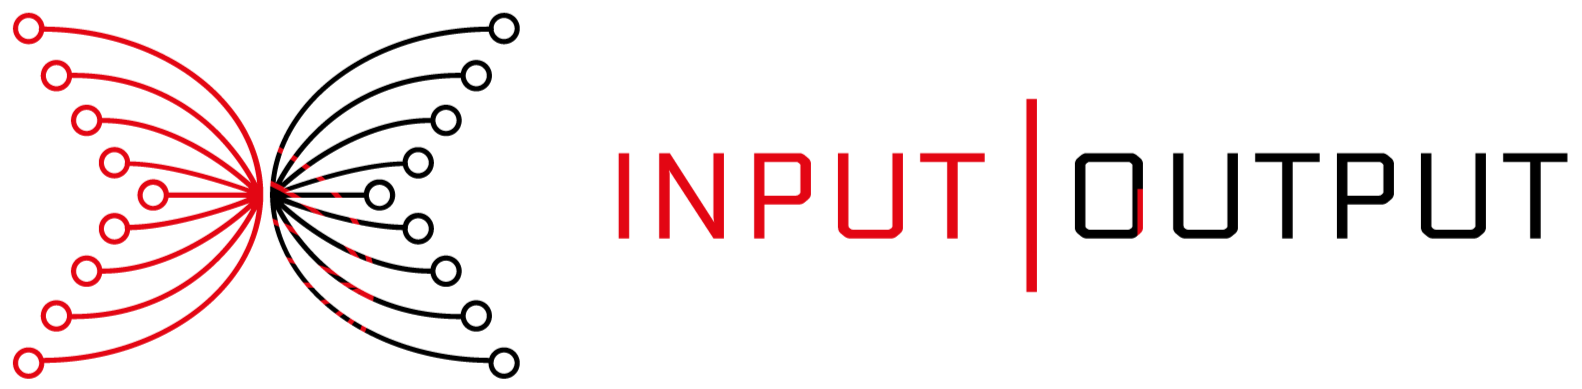
\includegraphics[keepaspectratio=true,height=1.4cm]{iohk}
}

\begin{document}
\begin{center}
\setbeamerfont{title}{size=\large}
\setbeamerfont{subtitle}{size=\small}
\maketitle
\setbeamerfont{title}{size=\Large}
\setbeamerfont{subtitle}{size=\large}
\end{center}

\section{Introduction}

\begin{frame}{Motivation}
\begin{itemize}
\item A lot of blockchain applications recently
\item Sophisticated transactional schemes via \alert{smart contracts}
\item Reasoning about their execution is:
  \begin{enumerate}
  \item \textit{necessary}, significant funds are involved
  \item \textit{difficult}, due to concurrency
  \end{enumerate}
\item Hence the need for automatic tools that verify no bugs exist
  \begin{itemize}
  \item This has to be done \alert{statically}!
  \end{itemize}
\end{itemize}
\end{frame}

\begin{frame}{Background}

\begin{alertblock}{Bitcoin}
\begin{itemize}
\item Based on \textit{unspent transaction outputs} (UTxO)
\item Smart contracts in the simple language \textsc{script}
\end{itemize}
\end{alertblock}

\begin{alertblock}{Ethereum}
\begin{itemize}
\item Based on the notion of accounts
\item Smart contracts in (almost) Turing-complete Solidity/EVM
\end{itemize}
\end{alertblock}

\begin{alertblock}{Cardano (IOHK)}
\begin{itemize}
\item UTxO-based, with several extensions
\item Due to the extensions, smart contracts become more expressive
\end{itemize}
\end{alertblock}

\end{frame}

\begin{frame}{Methodology}
\begin{itemize}
\item Keep things on an abstract level
  \begin{itemize}
  \item Setup long-term foundations
  \end{itemize}
\item Fully mechanized approach, utilizing Agda's rich type system
\item Fits well with IOHK's research-oriented approach
\end{itemize}

\begin{tikzpicture}
  [basic box/.style = {
     draw,
     shape = rectangle,
     align = center,
     minimum width=2cm,
     minimum height=1.2cm,
     rounded corners},
   to/.style = {
     ->,
     >=stealth',
     semithick
  },
  every matrix/.style={column sep=.8cm, ampersand replacement=\&},
  font=\small
  ]
  \matrix{
     \node[basic box] (a) {pure\\ research};
  \& \node[basic box] (b) {mechanized\\ models};
  \& \node[basic box] (c) {reference\\ implementations};
  \& \node[basic box] (d) {production\\ code}; \\
  };

  \path
  (a) edge[to, mLightBrown] (b)
  (b) edge[to] (c)
  (c) edge[to] (d)
  ;
\end{tikzpicture}
\end{frame}
\section{BitML}

\subsection{Contracts}

\begin{frame}{Basic Types}
\begin{agda}\begin{hscode}\SaveRestoreHook
\column{B}{@{}>{\hspre}l<{\hspost}@{}}%
\column{10}{@{}>{\hspre}l<{\hspost}@{}}%
\column{15}{@{}>{\hspre}l<{\hspost}@{}}%
\column{E}{@{}>{\hspre}l<{\hspost}@{}}%
\>[B]{}\HSKeyword{module}\;\HSCon{BitML}\;{}\<[15]%
\>[15]{}\HSSpecial{(}\HSCon{Participant}\mathbin{:}\HSCon{Set}\HSSpecial{)}\;{}\<[E]%
\\
\>[15]{}\HSSpecial{(}\HSSym{\anonymous}\HSSym{\mathbin{\overset{\text{\tiny ?}}{=}}}\HSSym{\textsub{p}}\;\HSSym{\anonymous}\mathbin{:}\HSCon{Decidable}\;\HSSpecial{\{\mskip1.5mu }\HSCon{A}\HSSym{\mathbin{=}}\HSCon{Participant}\HSSpecial{\mskip1.5mu\}}\;\HSSym{\anonymous}\HSSym{\mathrel{\equiv}}\HSSym{\anonymous}\HSSpecial{)}\;{}\<[E]%
\\
\>[15]{}\HSSpecial{(}\HSCon{Honest}\mathbin{:}\HSCon{List}\;\HSSym{\textsup{+}}\;\HSCon{Participant}\HSSpecial{)}\;\HSKeyword{where}{}\<[E]%
\\
\>[B]{}\HSCon{Time}{}\<[10]%
\>[10]{}\HSSym{\mathbin{=}}\HSSym{\mathbb{N}}{}\<[E]%
\\
\>[B]{}\HSCon{Value}{}\<[10]%
\>[10]{}\HSSym{\mathbin{=}}\HSSym{\mathbb{N}}{}\<[E]%
\\
\>[B]{}\HSCon{Secret}{}\<[10]%
\>[10]{}\HSSym{\mathbin{=}}\HSCon{String}{}\<[E]%
\\
\>[B]{}\HSCon{Deposit}{}\<[10]%
\>[10]{}\HSSym{\mathbin{=}}\HSCon{Participant}\HSSym{\mathrel{\times}}\HSCon{Value}{}\<[E]%
\ColumnHook
\end{hscode}\resethooks
\end{agda}
\end{frame}

\begin{frame}{Contract Preconditions}
\begin{agda}\begin{hscode}\SaveRestoreHook
\column{B}{@{}>{\hspre}l<{\hspost}@{}}%
\column{3}{@{}>{\hspre}l<{\hspost}@{}}%
\column{10}{@{}>{\hspre}c<{\hspost}@{}}%
\column{10E}{@{}l@{}}%
\column{13}{@{}>{\hspre}l<{\hspost}@{}}%
\column{20}{@{}>{\hspre}c<{\hspost}@{}}%
\column{20E}{@{}l@{}}%
\column{23}{@{}>{\hspre}l<{\hspost}@{}}%
\column{E}{@{}>{\hspre}l<{\hspost}@{}}%
\>[B]{}\HSKeyword{data}\;\HSCon{Precondition}{}\<[20]%
\>[20]{}\mathbin{:}{}\<[20E]%
\>[23]{}\HSCon{Values}\HSComment{ -\! - volatile deposits}{}\<[E]%
\\
\>[20]{}\HSSym{\mathbin{\to}}{}\<[20E]%
\>[23]{}\HSCon{Values}\HSComment{ -\! - persistent deposits}{}\<[E]%
\\
\>[20]{}\HSSym{\mathbin{\to}}{}\<[20E]%
\>[23]{}\HSCon{Set}\;\HSKeyword{where}{}\<[E]%
\\
\>[B]{}\hsindent{3}{}\<[3]%
\>[3]{}\HSComment{ -\! - volatile deposit}{}\<[E]%
\\
\>[B]{}\hsindent{3}{}\<[3]%
\>[3]{}\HSSym{\anonymous}\HSSym{?}\HSSym{\anonymous}\mathbin{:}\HSCon{Participant}\HSSym{\mathbin{\to}}\HSSpecial{(}\HSVar{v}\mathbin{:}\HSCon{Value}\HSSpecial{)}\HSSym{\mathbin{\to}}\HSCon{Precondition}\;\HSSpecial{[\mskip1.5mu }\HSVar{v}\HSSpecial{\mskip1.5mu]}\;\HSSpecial{[\mskip1.5mu }\HSSpecial{\mskip1.5mu]}{}\<[E]%
\\
\>[B]{}\hsindent{3}{}\<[3]%
\>[3]{}\HSComment{ -\! - persistent deposit}{}\<[E]%
\\
\>[B]{}\hsindent{3}{}\<[3]%
\>[3]{}\HSSym{\anonymous}\mathbin{!}\HSSym{\anonymous}\mathbin{:}\HSCon{Participant}\HSSym{\mathbin{\to}}\HSSpecial{(}\HSVar{v}\mathbin{:}\HSCon{Value}\HSSpecial{)}\HSSym{\mathbin{\to}}\HSCon{Precondition}\;\HSSpecial{[\mskip1.5mu }\HSSpecial{\mskip1.5mu]}\;\HSSpecial{[\mskip1.5mu }\HSVar{v}\HSSpecial{\mskip1.5mu]}{}\<[E]%
\\
\>[B]{}\hsindent{3}{}\<[3]%
\>[3]{}\HSComment{ -\! - committed secret}{}\<[E]%
\\
\>[B]{}\hsindent{3}{}\<[3]%
\>[3]{}\HSSym{\anonymous}\HSSym{\hspace{1pt}\#}\HSSym{\anonymous}\mathbin{:}\HSCon{Participant}\HSSym{\mathbin{\to}}\HSCon{Secret}\HSSym{\mathbin{\to}}\HSCon{Precondition}\;\HSSpecial{[\mskip1.5mu }\HSSpecial{\mskip1.5mu]}\;\HSSpecial{[\mskip1.5mu }\HSSpecial{\mskip1.5mu]}{}\<[E]%
\\
\>[B]{}\hsindent{3}{}\<[3]%
\>[3]{}\HSComment{ -\! - conjunction}{}\<[E]%
\\
\>[B]{}\hsindent{3}{}\<[3]%
\>[3]{}\HSSym{\anonymous}\HSSym{\mathbin{\land}}\HSSym{\anonymous}{}\<[10]%
\>[10]{}\mathbin{:}{}\<[10E]%
\>[13]{}\HSCon{Precondition}\;\HSVar{vs}\;\HSSym{\textsub{v}}\;\HSVar{vs}\;\HSSym{\textsub{p}}\HSSym{\mathbin{\to}}\HSCon{Precondition}\;\HSVar{vs}\;\HSSym{\textsub{v}}\;\! ^{\prime}\;\HSVar{vs}\;\HSSym{\textsub{p}}\;\! ^{\prime}{}\<[E]%
\\
\>[10]{}\HSSym{\mathbin{\to}}{}\<[10E]%
\>[13]{}\HSCon{Precondition}\;\HSSpecial{(}\HSVar{vs}\;\HSSym{\textsub{v}}\HSSym{\mathbin{\plus}}\HSVar{vs}\;\HSSym{\textsub{v}}\;\! ^{\prime}\HSSpecial{)}\;\HSSpecial{(}\HSVar{vs}\;\HSSym{\textsub{p}}\HSSym{\mathbin{\plus}}\HSVar{vs}\;\HSSym{\textsub{p}}\;\! ^{\prime}\HSSpecial{)}{}\<[E]%
\ColumnHook
\end{hscode}\resethooks
\end{agda}
\end{frame}

\begin{frame}{Contracts I}
\savecolumns
\begin{agda}\begin{hscode}\SaveRestoreHook
\column{B}{@{}>{\hspre}l<{\hspost}@{}}%
\column{3}{@{}>{\hspre}l<{\hspost}@{}}%
\column{5}{@{}>{\hspre}c<{\hspost}@{}}%
\column{5E}{@{}l@{}}%
\column{8}{@{}>{\hspre}l<{\hspost}@{}}%
\column{16}{@{}>{\hspre}c<{\hspost}@{}}%
\column{16E}{@{}l@{}}%
\column{19}{@{}>{\hspre}l<{\hspost}@{}}%
\column{27}{@{}>{\hspre}l<{\hspost}@{}}%
\column{E}{@{}>{\hspre}l<{\hspost}@{}}%
\>[B]{}\HSKeyword{data}\;\HSCon{Contract}{}\<[16]%
\>[16]{}\mathbin{:}{}\<[16E]%
\>[19]{}\HSCon{Value}{}\<[27]%
\>[27]{}\HSComment{ -\! - the monetary value it carries}{}\<[E]%
\\
\>[16]{}\HSSym{\mathbin{\to}}{}\<[16E]%
\>[19]{}\HSCon{Values}{}\<[27]%
\>[27]{}\HSComment{ -\! - the volatile deposits it presumes}{}\<[E]%
\\
\>[16]{}\HSSym{\mathbin{\to}}{}\<[16E]%
\>[19]{}\HSCon{Set}\;\HSKeyword{where}{}\<[E]%
\\[\blanklineskip]%
\>[B]{}\hsindent{3}{}\<[3]%
\>[3]{}\HSComment{ -\! - collect deposits and secrets}{}\<[E]%
\\
\>[B]{}\hsindent{3}{}\<[3]%
\>[3]{}\HSVar{put}\;\HSSym{\anonymous}\;\HSVar{reveal}\;\HSSym{\anonymous}\;if\;\HSSym{\anonymous}\HSSym{\mathrel{\Rightarrow}}\HSSym{\anonymous}\HSSym{\dashv}\HSSym{\anonymous}\mathbin{:}{}\<[E]%
\\
\>[3]{}\hsindent{5}{}\<[8]%
\>[8]{}\HSSpecial{(}\HSVar{vs}\mathbin{:}\HSCon{Values}\HSSpecial{)}\HSSym{\mathbin{\to}}\HSSpecial{(}\HSVar{s}\mathbin{:}\HSCon{Secrets}\HSSpecial{)}\HSSym{\mathbin{\to}}\HSCon{Predicate}\;\HSVar{s}\;\! ^{\prime}{}\<[E]%
\\
\>[3]{}\hsindent{2}{}\<[5]%
\>[5]{}\HSSym{\mathbin{\to}}{}\<[5E]%
\>[8]{}\HSCon{Contract}\;\HSSpecial{(}\HSVar{v}\HSSym{+}\HSVar{sum}\;\HSVar{vs}\HSSpecial{)}\;\HSVar{vs}\;\! ^{\prime}\HSSym{\mathbin{\to}}\HSVar{s}\;\! ^{\prime}\HSSym{\mathrel{\subseteq}}\HSVar{s}{}\<[E]%
\\
\>[3]{}\hsindent{2}{}\<[5]%
\>[5]{}\HSSym{\mathbin{\to}}{}\<[5E]%
\>[8]{}\HSCon{Contract}\;\HSVar{v}\;\HSSpecial{(}\HSVar{vs}\;\! ^{\prime}\HSSym{\mathbin{\plus}}\HSVar{vs}\HSSpecial{)}{}\<[E]%
\\[\blanklineskip]%
\>[B]{}\hsindent{3}{}\<[3]%
\>[3]{}\HSComment{ -\! - transfer the remaining balance to a participant}{}\<[E]%
\\
\>[B]{}\hsindent{3}{}\<[3]%
\>[3]{}\HSVar{withdraw}\mathbin{:}\HSSym{\forall\ }\HSSpecial{\{\mskip1.5mu }\HSVar{v}\;\HSVar{vs}\HSSpecial{\mskip1.5mu\}}\HSSym{\mathbin{\to}}\HSCon{Participant}\HSSym{\mathbin{\to}}\HSCon{Contract}\;\HSVar{v}\;\HSVar{vs}{}\<[E]%
\ColumnHook
\end{hscode}\resethooks
\end{agda}
\end{frame}

\begin{frame}{Contracts II}
\restorecolumns
\begin{agda}\begin{hscode}\SaveRestoreHook
\column{B}{@{}>{\hspre}l<{\hspost}@{}}%
\column{3}{@{}>{\hspre}l<{\hspost}@{}}%
\column{9}{@{}>{\hspre}c<{\hspost}@{}}%
\column{9E}{@{}l@{}}%
\column{12}{@{}>{\hspre}l<{\hspost}@{}}%
\column{E}{@{}>{\hspre}l<{\hspost}@{}}%
\>[3]{}\HSComment{ -\! - split the balance across different branches}{}\<[E]%
\\
\>[3]{}\HSVar{split}\mathbin{:}{}\<[12]%
\>[12]{}\HSSym{\forall\ }\HSSpecial{\{\mskip1.5mu }\HSVar{vs}\HSSpecial{\mskip1.5mu\}}\HSSym{\mathbin{\to}}\HSSpecial{(}\HSVar{cs}\mathbin{:}\HSCon{List}\;\HSSpecial{(}\HSSym{\exists}\HSSpecial{[\mskip1.5mu }\HSVar{v}\HSSpecial{\mskip1.5mu]}\;\HSCon{Contract}\;\HSVar{v}\;\HSVar{vs}\HSSpecial{)}\HSSpecial{)}{}\<[E]%
\\
\>[3]{}\hsindent{6}{}\<[9]%
\>[9]{}\HSSym{\mathbin{\to}}{}\<[9E]%
\>[12]{}\HSCon{Contract}\;\HSSpecial{(}\HSVar{sum}\;\HSSpecial{(}\HSVar{proj}\;\textsub{1}\HSSym{\mathrel{\langle\$\rangle}}\HSVar{cs}\HSSpecial{)}\HSSpecial{)}\;\HSVar{vs}{}\<[E]%
\\[\blanklineskip]%
\>[3]{}\HSComment{ -\! - wait for participant's authorization}{}\<[E]%
\\
\>[3]{}\HSSym{\anonymous}\HSSym{\mathbin{:}}\HSSym{\anonymous}\mathbin{:}\HSCon{Participant}\HSSym{\mathbin{\to}}\HSCon{Contract}\;\HSVar{v}\;\HSVar{vs}\HSSym{\mathbin{\to}}\HSCon{Contract}\;\HSVar{v}\;\HSVar{vs}{}\<[E]%
\\[\blanklineskip]%
\>[3]{}\HSComment{ -\! - wait until some time passes}{}\<[E]%
\\
\>[3]{}\HSVar{after}\;\HSSym{\anonymous}\mathbin{:}\HSSym{\anonymous}\mathbin{:}\HSCon{Time}\HSSym{\mathbin{\to}}\HSCon{Contract}\;\HSVar{v}\;\HSVar{vs}\HSSym{\mathbin{\to}}\HSCon{Contract}\;\HSVar{v}\;\HSVar{vs}{}\<[E]%
\ColumnHook
\end{hscode}\resethooks
\end{agda}
\end{frame}

\begin{frame}{Advertisements}
\begin{agda}\begin{hscode}\SaveRestoreHook
\column{B}{@{}>{\hspre}l<{\hspost}@{}}%
\column{3}{@{}>{\hspre}l<{\hspost}@{}}%
\column{10}{@{}>{\hspre}l<{\hspost}@{}}%
\column{17}{@{}>{\hspre}c<{\hspost}@{}}%
\column{17E}{@{}l@{}}%
\column{20}{@{}>{\hspre}l<{\hspost}@{}}%
\column{22}{@{}>{\hspre}c<{\hspost}@{}}%
\column{22E}{@{}l@{}}%
\column{E}{@{}>{\hspre}l<{\hspost}@{}}%
\>[B]{}\HSKeyword{record}\;\HSCon{Advertisement}\;\HSSpecial{(}\HSVar{v}\mathbin{:}\HSCon{Value}\HSSpecial{)}\;\HSSpecial{(}\HSVar{vs}\;\HSSym{\textsup{c}}\;\HSVar{vs}\;\HSSym{\textsup{v}}\;\HSVar{vs}\;\HSSym{\textsup{p}}\mathbin{:}\HSCon{Values}\HSSpecial{)}\mathbin{:}\HSCon{Set}\;\HSKeyword{where}{}\<[E]%
\\
\>[B]{}\hsindent{3}{}\<[3]%
\>[3]{}\HSKeyword{constructor}\;\HSSym{\anonymous}\HSSym{\langle\ }\HSSym{\anonymous}\HSSym{\ \rangle\dashv}\HSSym{\anonymous}{}\<[E]%
\\
\>[B]{}\hsindent{3}{}\<[3]%
\>[3]{}\HSKeyword{field}\;{}\<[10]%
\>[10]{}\HSCon{G}{}\<[17]%
\>[17]{}\mathbin{:}{}\<[17E]%
\>[20]{}\HSCon{Precondition}\;\HSVar{vs}\;\HSSym{\textsup{v}}\;\HSVar{vs}\;\HSSym{\textsup{p}}{}\<[E]%
\\
\>[10]{}\HSCon{C}{}\<[17]%
\>[17]{}\mathbin{:}{}\<[17E]%
\>[20]{}\HSCon{Contracts}\;\HSVar{v}\;\HSVar{vs}\;\HSSym{\textsup{c}}{}\<[E]%
\\
\>[10]{}\HSVar{valid}{}\<[17]%
\>[17]{}\mathbin{:}{}\<[17E]%
\>[20]{}\HSVar{length}\;\HSVar{vs}\;\HSSym{\textsup{c}}\HSSym{\mathrel{\leq}}\HSVar{length}\;\HSVar{vs}\;\HSSym{\textsup{v}}{}\<[E]%
\\
\>[17]{}\HSSym{\mathrel{\times}}{}\<[17E]%
\>[20]{}\HSVar{participants}\;\HSSym{\textsup{g}}\;\HSCon{G}\HSSym{\mathbin{\plus}}\HSVar{participants}\;\HSSym{\textsup{c}}\;\HSCon{C}{}\<[E]%
\\
\>[20]{}\hsindent{2}{}\<[22]%
\>[22]{}\HSSym{\mathrel{\subseteq}}{}\<[22E]%
\\
\>[20]{}\HSVar{participant}\HSSym{\mathrel{\langle\$\rangle}}\HSVar{persistentDeposits}\;\HSCon{G}{}\<[E]%
\\
\>[17]{}\HSSym{\mathrel{\times}}{}\<[17E]%
\>[20]{}\HSVar{v}\HSSym{\mathrel{\equiv}}\HSVar{sum}\;\HSVar{vs}\;\HSSym{\textsup{p}}{}\<[E]%
\ColumnHook
\end{hscode}\resethooks
\end{agda}
\end{frame}

\begin{frame}{Example Advertisement}
\begin{agda}\begin{hscode}\SaveRestoreHook
\column{B}{@{}>{\hspre}l<{\hspost}@{}}%
\column{10}{@{}>{\hspre}c<{\hspost}@{}}%
\column{10E}{@{}l@{}}%
\column{11}{@{}>{\hspre}l<{\hspost}@{}}%
\column{13}{@{}>{\hspre}l<{\hspost}@{}}%
\column{18}{@{}>{\hspre}c<{\hspost}@{}}%
\column{18E}{@{}l@{}}%
\column{21}{@{}>{\hspre}l<{\hspost}@{}}%
\column{E}{@{}>{\hspre}l<{\hspost}@{}}%
\>[B]{}\HSKeyword{open}\;\HSCon{BitML}\;\HSSpecial{(}\HSCon{A}\HSSym{\mathbin{\mid}}\HSCon{B}\HSSpecial{)}\;\HSSym{\dots}\;\HSSpecial{[\mskip1.5mu }\HSCon{A}\HSSpecial{\mskip1.5mu]}\;\HSSym{\textsup{+}}{}\<[E]%
\\[\blanklineskip]%
\>[B]{}\HSVar{ex}\HSSym{\text{\textit{-}}}\HSVar{ad}\mathbin{:}\HSCon{Advertisement}\;\HSNumeral{5}\;\HSSpecial{[\mskip1.5mu }\HSNumeral{200}\HSSpecial{\mskip1.5mu]}\;\HSSpecial{[\mskip1.5mu }\HSNumeral{200}\HSSpecial{\mskip1.5mu]}\;\HSSpecial{[\mskip1.5mu }\HSNumeral{3}\HSSpecial{\HSSym{\mathbin{,}}}\HSNumeral{2}\HSSpecial{\mskip1.5mu]}{}\<[E]%
\\
\>[B]{}\HSVar{ex}\HSSym{\text{\textit{-}}}\HSVar{ad}\HSSym{\mathbin{=}}{}\<[10]%
\>[10]{}\HSSym{\langle\ }{}\<[10E]%
\>[13]{}\HSCon{B}\mathbin{!}\HSNumeral{3}\HSSym{\mathbin{\land}}\HSCon{A}\mathbin{!}\HSNumeral{2}\HSSym{\mathbin{\land}}\HSCon{A}\HSSym{?}\HSNumeral{200}\HSSym{\ \rangle}{}\<[E]%
\\
\>[10]{}\hsindent{1}{}\<[11]%
\>[11]{}\HSVar{split}\;{}\<[18]%
\>[18]{}\HSSpecial{(}{}\<[18E]%
\>[21]{}\HSNumeral{2}\HSSym{\multimap}\HSVar{withdraw}\;\HSCon{B}{}\<[E]%
\\
\>[18]{}\HSSym{\mathbin{\oplus}}{}\<[18E]%
\>[21]{}\HSNumeral{2}\HSSym{\multimap}\HSVar{after}\;\HSNumeral{42}\HSSym{\mathbin{:}}\HSVar{withdraw}\;\HSCon{A}{}\<[E]%
\\
\>[18]{}\HSSym{\mathbin{\oplus}}{}\<[18E]%
\>[21]{}\HSNumeral{1}\HSSym{\multimap}\HSVar{put}\;\HSSpecial{[\mskip1.5mu }\HSNumeral{200}\HSSpecial{\mskip1.5mu]}\HSSym{\mathrel{\Rightarrow}}\HSCon{B}\HSSym{\mathbin{:}}\HSVar{withdraw}\;\HSSpecial{\{\mskip1.5mu }\HSNumeral{201}\HSSpecial{\mskip1.5mu\}}\;\HSCon{A}\;\HSSpecial{)}{}\<[E]%
\\
\>[10]{}\hsindent{1}{}\<[11]%
\>[11]{}\HSSym{\dashv}\HSSym{\dots}{}\<[E]%
\ColumnHook
\end{hscode}\resethooks
\end{agda}
\end{frame}

\subsection{Small-step Semantics}

\begin{frame}{Small-step Semantics: Actions I}
\begin{agda}\begin{hscode}\SaveRestoreHook
\column{B}{@{}>{\hspre}l<{\hspost}@{}}%
\column{3}{@{}>{\hspre}c<{\hspost}@{}}%
\column{3E}{@{}l@{}}%
\column{6}{@{}>{\hspre}l<{\hspost}@{}}%
\column{22}{@{}>{\hspre}l<{\hspost}@{}}%
\column{32}{@{}>{\hspre}l<{\hspost}@{}}%
\column{E}{@{}>{\hspre}l<{\hspost}@{}}%
\>[B]{}\HSCon{AdvertisedContracts}{}\<[22]%
\>[22]{}\HSSym{\mathbin{=}}\HSCon{List}\;\HSSpecial{(}\HSSym{\exists}\HSSpecial{[\mskip1.5mu }\HSVar{v}\HSSpecial{\HSSym{\mathbin{,}}}\HSSym{\dots}\HSSpecial{\HSSym{\mathbin{,}}}\HSVar{vs}\;\HSSym{\textsup{p}}\HSSpecial{\mskip1.5mu]}\;\HSCon{Advertisement}\;\HSVar{v}\;\HSSym{\dots}\;\HSVar{vs}\;\HSSym{\textsup{p}}\HSSpecial{)}{}\<[E]%
\\
\>[B]{}\HSCon{ActiveContracts}{}\<[22]%
\>[22]{}\HSSym{\mathbin{=}}\HSCon{List}\;\HSSpecial{(}\HSSym{\exists}\HSSpecial{[\mskip1.5mu }\HSVar{v}\HSSpecial{\HSSym{\mathbin{,}}}\HSVar{vs}\HSSpecial{\mskip1.5mu]}\;\HSCon{Contracts}\;\HSVar{v}\;\HSVar{vs}\HSSpecial{)}{}\<[E]%
\\
\>[B]{}\vspace{1pt}{}\<[E]%
\\
\>[B]{}\HSKeyword{data}\;\HSCon{Action}\;\HSSpecial{(}\HSVar{p}\mathbin{:}\HSCon{Participant}\HSSpecial{)}{}\<[32]%
\>[32]{}\HSComment{ -\! - the participant that authorizes this action}{}\<[E]%
\\
\>[B]{}\hsindent{3}{}\<[3]%
\>[3]{}\mathbin{:}{}\<[3E]%
\>[6]{}\HSCon{AdvertisedContracts}{}\<[32]%
\>[32]{}\HSComment{ -\! - contract advertisements it requires}{}\<[E]%
\\
\>[B]{}\hsindent{3}{}\<[3]%
\>[3]{}\HSSym{\mathbin{\to}}{}\<[3E]%
\>[6]{}\HSCon{ActiveContracts}{}\<[32]%
\>[32]{}\HSComment{ -\! - active contracts it requires}{}\<[E]%
\\
\>[B]{}\hsindent{3}{}\<[3]%
\>[3]{}\HSSym{\mathbin{\to}}{}\<[3E]%
\>[6]{}\HSCon{Values}{}\<[32]%
\>[32]{}\HSComment{ -\! - deposits it requires from the participant}{}\<[E]%
\\
\>[B]{}\hsindent{3}{}\<[3]%
\>[3]{}\HSSym{\mathbin{\to}}{}\<[3E]%
\>[6]{}\HSCon{Deposits}{}\<[32]%
\>[32]{}\HSComment{ -\! - deposits it produces}{}\<[E]%
\\
\>[B]{}\hsindent{3}{}\<[3]%
\>[3]{}\HSSym{\mathbin{\to}}{}\<[3E]%
\>[6]{}\HSCon{Set}\;\HSKeyword{where}{}\<[E]%
\ColumnHook
\end{hscode}\resethooks
\end{agda}
\end{frame}

\begin{frame}{Small-step Semantics: Actions II}
\begin{agda}\begin{hscode}\SaveRestoreHook
\column{B}{@{}>{\hspre}l<{\hspost}@{}}%
\column{3}{@{}>{\hspre}l<{\hspost}@{}}%
\column{10}{@{}>{\hspre}l<{\hspost}@{}}%
\column{11}{@{}>{\hspre}l<{\hspost}@{}}%
\column{13}{@{}>{\hspre}l<{\hspost}@{}}%
\column{14}{@{}>{\hspre}l<{\hspost}@{}}%
\column{22}{@{}>{\hspre}l<{\hspost}@{}}%
\column{40}{@{}>{\hspre}l<{\hspost}@{}}%
\column{E}{@{}>{\hspre}l<{\hspost}@{}}%
\>[3]{}\HSComment{ -\! - join two deposits}{}\<[E]%
\\
\>[3]{}\HSSym{\anonymous}\HSSym{\mathrel{\leftrightarrow}}\HSSym{\anonymous}{}\<[10]%
\>[10]{}\mathbin{:}\HSSym{\forall\ }\HSSpecial{\{\mskip1.5mu }\HSVar{vs}\HSSpecial{\mskip1.5mu\}}\HSSym{\mathbin{\to}}{}\<[22]%
\>[22]{}\HSSpecial{(}\HSVar{i}\mathbin{:}\HSCon{Index}\;\HSVar{vs}\HSSpecial{)}\HSSym{\mathbin{\to}}{}\<[40]%
\>[40]{}\HSSpecial{(}\HSVar{j}\mathbin{:}\HSCon{Index}\;\HSVar{vs}\HSSpecial{)}{}\<[E]%
\\
\>[10]{}\HSSym{\mathbin{\to}}\HSCon{Action}\;\HSVar{p}\;\HSSpecial{[\mskip1.5mu }\HSSpecial{\mskip1.5mu]}\;\HSSpecial{[\mskip1.5mu }\HSSpecial{\mskip1.5mu]}\;\HSVar{vs}\;\HSSpecial{(}\HSVar{p}\;\HSVar{has}\;\HSSym{\!\_}\;\HSSym{\mathrel{\langle\$\rangle}}\HSVar{merge}\;\HSVar{i}\;\HSVar{j}\;\HSVar{vs}\HSSpecial{)}{}\<[E]%
\\
\>[3]{}\HSComment{ -\! - commit secrets to stipulate an advertisement}{}\<[E]%
\\
\>[3]{}\HSSym{\#\!\vartriangleright\!\!}\;\HSSym{\anonymous}{}\<[11]%
\>[11]{}\mathbin{:}\HSSpecial{(}\HSVar{ad}\mathbin{:}\HSCon{Advertisement}\;\HSVar{v}\;\HSVar{vs}\;\HSSym{\textsup{c}}\;\HSVar{vs}\;\HSSym{\textsup{v}}\;\HSVar{vs}\;\HSSym{\textsup{p}}\HSSpecial{)}{}\<[E]%
\\
\>[11]{}\HSSym{\mathbin{\to}}\HSCon{Action}\;\HSVar{p}\;\HSSpecial{[\mskip1.5mu }\HSVar{v}\HSSpecial{\HSSym{\mathbin{,}}}\HSVar{vs}\;\HSSym{\textsup{c}}\HSSpecial{\HSSym{\mathbin{,}}}\HSVar{vs}\;\HSSym{\textsup{v}}\HSSpecial{\HSSym{\mathbin{,}}}\HSVar{vs}\;\HSSym{\textsup{p}}\HSSpecial{\HSSym{\mathbin{,}}}\HSVar{ad}\HSSpecial{\mskip1.5mu]}\;\HSSpecial{[\mskip1.5mu }\HSSpecial{\mskip1.5mu]}\;\HSSpecial{[\mskip1.5mu }\HSSpecial{\mskip1.5mu]}\;\HSSpecial{[\mskip1.5mu }\HSSpecial{\mskip1.5mu]}{}\<[E]%
\\
\>[3]{}\HSComment{ -\! - spend x to stipulate an advertisement}{}\<[E]%
\\
\>[3]{}\HSSym{\anonymous}\;\HSSym{{\vartriangleright}^s}\;\HSSym{\anonymous}{}\<[13]%
\>[13]{}\mathbin{:}\HSSpecial{(}\HSVar{ad}\mathbin{:}\HSCon{Advertisement}\;\HSVar{v}\;\HSVar{vs}\;\HSSym{\textsup{c}}\;\HSVar{vs}\;\HSSym{\textsup{v}}\;\HSVar{vs}\;\HSSym{\textsup{p}}\HSSpecial{)}\HSSym{\mathbin{\to}}\HSSpecial{(}\HSVar{i}\mathbin{:}\HSCon{Index}\;\HSVar{vs}\;\HSSym{\textsup{p}}\HSSpecial{)}{}\<[E]%
\\
\>[13]{}\HSSym{\mathbin{\to}}\HSCon{Action}\;\HSVar{p}\;\HSSpecial{[\mskip1.5mu }\HSVar{v}\HSSpecial{\HSSym{\mathbin{,}}}\HSVar{vs}\;\HSSym{\textsup{c}}\HSSpecial{\HSSym{\mathbin{,}}}\HSVar{vs}\;\HSSym{\textsup{v}}\HSSpecial{\HSSym{\mathbin{,}}}\HSVar{vs}\;\HSSym{\textsup{p}}\HSSpecial{\HSSym{\mathbin{,}}}\HSVar{ad}\HSSpecial{\mskip1.5mu]}\;\HSSpecial{[\mskip1.5mu }\HSSpecial{\mskip1.5mu]}\;\HSSpecial{[\mskip1.5mu }\HSVar{vs}\;\HSSym{\textsup{p}}\HSSym{\mathbin{!!}}\HSVar{i}\HSSpecial{\mskip1.5mu]}\;\HSSpecial{[\mskip1.5mu }\HSSpecial{\mskip1.5mu]}{}\<[E]%
\\
\>[3]{}\HSComment{ -\! - pick a branch}{}\<[E]%
\\
\>[3]{}\HSSym{\anonymous}\;\HSSym{{\vartriangleright}^b}\;\HSSym{\anonymous}{}\<[14]%
\>[14]{}\mathbin{:}\HSSpecial{(}\HSVar{c}\mathbin{:}\HSCon{Contracts}\;\HSVar{v}\;\HSVar{vs}\HSSpecial{)}\HSSym{\mathbin{\to}}\HSSpecial{(}\HSVar{i}\mathbin{:}\HSCon{Index}\;\HSVar{c}\HSSpecial{)}{}\<[E]%
\\
\>[14]{}\HSSym{\mathbin{\to}}\HSCon{Action}\;\HSVar{p}\;\HSSpecial{[\mskip1.5mu }\HSSpecial{\mskip1.5mu]}\;\HSSpecial{[\mskip1.5mu }\HSVar{v}\HSSpecial{\HSSym{\mathbin{,}}}\HSVar{vs}\HSSpecial{\HSSym{\mathbin{,}}}\HSVar{c}\HSSpecial{\mskip1.5mu]}\;\HSSpecial{[\mskip1.5mu }\HSSpecial{\mskip1.5mu]}\;\HSSpecial{[\mskip1.5mu }\HSSpecial{\mskip1.5mu]}{}\<[E]%
\\
\>[3]{}\HSSym{\vdots}{}\<[E]%
\ColumnHook
\end{hscode}\resethooks
\end{agda}
\end{frame}

\begin{frame}{Small-step Semantics: Actions Example}
\begin{agda}\begin{hscode}\SaveRestoreHook
\column{B}{@{}>{\hspre}l<{\hspost}@{}}%
\column{E}{@{}>{\hspre}l<{\hspost}@{}}%
\>[B]{}\HSComment{ -\! - A spends the required {\bitcoin~ 2}, as stated in the pre-condition}{}\<[E]%
\\
\>[B]{}\HSVar{ex}\HSSym{\text{\textit{-}}}\HSVar{spend}\mathbin{:}\HSCon{Action}\;\HSCon{A}\;\HSSpecial{[\mskip1.5mu }\HSNumeral{5}\HSSpecial{\HSSym{\mathbin{,}}}\HSSpecial{[\mskip1.5mu }\HSNumeral{200}\HSSpecial{\mskip1.5mu]}\HSSpecial{\HSSym{\mathbin{,}}}\HSSpecial{[\mskip1.5mu }\HSNumeral{200}\HSSpecial{\mskip1.5mu]}\HSSpecial{\HSSym{\mathbin{,}}}\HSSpecial{[\mskip1.5mu }\HSNumeral{3}\HSSpecial{\HSSym{\mathbin{,}}}\HSNumeral{2}\HSSpecial{\mskip1.5mu]}\HSSpecial{\HSSym{\mathbin{,}}}\HSVar{ex}\HSSym{\text{\textit{-}}}\HSVar{ad}\HSSpecial{\mskip1.5mu]}\;\HSSpecial{[\mskip1.5mu }\HSSpecial{\mskip1.5mu]}\;\HSSpecial{[\mskip1.5mu }\HSNumeral{2}\HSSpecial{\mskip1.5mu]}\;\HSSpecial{[\mskip1.5mu }\HSSpecial{\mskip1.5mu]}{}\<[E]%
\\
\>[B]{}\HSVar{ex}\HSSym{\text{\textit{-}}}\HSVar{spend}\HSSym{\mathbin{=}}\HSVar{ex}\HSSym{\text{\textit{-}}}\HSVar{ad}\;\HSSym{{\vartriangleright}^s}\;\HSNumeral{1}{}\<[E]%
\ColumnHook
\end{hscode}\resethooks
\end{agda}
\end{frame}

\begin{frame}{Small-step Semantics: Configurations I}
\begin{agda}\begin{hscode}\SaveRestoreHook
\column{B}{@{}>{\hspre}l<{\hspost}@{}}%
\column{3}{@{}>{\hspre}l<{\hspost}@{}}%
\column{8}{@{}>{\hspre}l<{\hspost}@{}}%
\column{18}{@{}>{\hspre}l<{\hspost}@{}}%
\column{27}{@{}>{\hspre}c<{\hspost}@{}}%
\column{27E}{@{}l@{}}%
\column{30}{@{}>{\hspre}l<{\hspost}@{}}%
\column{51}{@{}>{\hspre}l<{\hspost}@{}}%
\column{E}{@{}>{\hspre}l<{\hspost}@{}}%
\>[B]{}\HSKeyword{data}\;\HSCon{Configuration}\;\! ^{\prime}{}\<[27]%
\>[27]{}\mathbin{:}{}\<[27E]%
\>[30]{}\HSComment{ -\! - $\hspace{19pt}$ current $\hspace{19pt}$ $\times$ $\hspace{19pt}$ required}{}\<[E]%
\\
\>[30]{}\HSCon{AdvertisedContracts}{}\<[51]%
\>[51]{}\HSSym{\mathrel{\times}}\HSCon{AdvertisedContracts}{}\<[E]%
\\
\>[27]{}\HSSym{\mathbin{\to}}{}\<[27E]%
\>[30]{}\HSCon{ActiveContracts}{}\<[51]%
\>[51]{}\HSSym{\mathrel{\times}}\HSCon{ActiveContracts}{}\<[E]%
\\
\>[27]{}\HSSym{\mathbin{\to}}{}\<[27E]%
\>[30]{}\HSCon{Deposits}{}\<[51]%
\>[51]{}\HSSym{\mathrel{\times}}\HSCon{Deposits}{}\<[E]%
\\
\>[27]{}\HSSym{\mathbin{\to}}{}\<[27E]%
\>[30]{}\HSCon{Set}\;\HSKeyword{where}{}\<[E]%
\\[\blanklineskip]%
\>[B]{}\hsindent{3}{}\<[3]%
\>[3]{}\HSComment{ -\! - empty}{}\<[E]%
\\
\>[B]{}\hsindent{3}{}\<[3]%
\>[3]{}\HSSym{\varnothing}\mathbin{:}\HSCon{Configuration}\;\! ^{\prime}\;\HSSpecial{(}\HSSpecial{[\mskip1.5mu }\HSSpecial{\mskip1.5mu]}\HSSpecial{\HSSym{\mathbin{,}}}\HSSpecial{[\mskip1.5mu }\HSSpecial{\mskip1.5mu]}\HSSpecial{)}\;\HSSpecial{(}\HSSpecial{[\mskip1.5mu }\HSSpecial{\mskip1.5mu]}\HSSpecial{\HSSym{\mathbin{,}}}\HSSpecial{[\mskip1.5mu }\HSSpecial{\mskip1.5mu]}\HSSpecial{)}\;\HSSpecial{(}\HSSpecial{[\mskip1.5mu }\HSSpecial{\mskip1.5mu]}\HSSpecial{\HSSym{\mathbin{,}}}\HSSpecial{[\mskip1.5mu }\HSSpecial{\mskip1.5mu]}\HSSpecial{)}{}\<[E]%
\\[\blanklineskip]%
\>[B]{}\hsindent{3}{}\<[3]%
\>[3]{}\HSComment{ -\! - contract advertisement}{}\<[E]%
\\
\>[B]{}\hsindent{3}{}\<[3]%
\>[3]{}\HSSpecial{`}\HSSym{\anonymous}{}\<[8]%
\>[8]{}\mathbin{:}\HSSpecial{(}\HSVar{ad}\mathbin{:}\HSCon{Advertisement}\;\HSVar{v}\;\HSVar{vs}\;\HSSym{\textsup{c}}\;\HSVar{vs}\;\HSSym{\textsup{v}}\;\HSVar{vs}\;\HSSym{\textsup{p}}\HSSpecial{)}{}\<[E]%
\\
\>[8]{}\HSSym{\mathbin{\to}}\HSCon{Configuration}\;\! ^{\prime}\;\HSSpecial{(}\HSSpecial{[\mskip1.5mu }\HSVar{v}\HSSpecial{\HSSym{\mathbin{,}}}\HSVar{vs}\;\HSSym{\textsup{c}}\HSSpecial{\HSSym{\mathbin{,}}}\HSVar{vs}\;\HSSym{\textsup{v}}\HSSpecial{\HSSym{\mathbin{,}}}\HSVar{vs}\;\HSSym{\textsup{p}}\HSSpecial{\HSSym{\mathbin{,}}}\HSVar{ad}\HSSpecial{\mskip1.5mu]}\HSSpecial{\HSSym{\mathbin{,}}}\HSSpecial{[\mskip1.5mu }\HSSpecial{\mskip1.5mu]}\HSSpecial{)}\;\HSSpecial{(}\HSSpecial{[\mskip1.5mu }\HSSpecial{\mskip1.5mu]}\HSSpecial{\HSSym{\mathbin{,}}}\HSSpecial{[\mskip1.5mu }\HSSpecial{\mskip1.5mu]}\HSSpecial{)}\;\HSSpecial{(}\HSSpecial{[\mskip1.5mu }\HSSpecial{\mskip1.5mu]}\HSSpecial{\HSSym{\mathbin{,}}}\HSSpecial{[\mskip1.5mu }\HSSpecial{\mskip1.5mu]}\HSSpecial{)}{}\<[E]%
\\[\blanklineskip]%
\>[B]{}\hsindent{3}{}\<[3]%
\>[3]{}\HSComment{ -\! - active contract}{}\<[E]%
\\
\>[B]{}\hsindent{3}{}\<[3]%
\>[3]{}\HSSym{\langle\ }\HSSym{\anonymous}\HSSpecial{\HSSym{\mathbin{,}}}\HSSym{\anonymous}\HSSym{\ \rangle}\HSSym{\ \textsup{c}}{}\<[18]%
\>[18]{}\mathbin{:}\HSSpecial{(}\HSVar{c}\mathbin{:}\HSCon{Contracts}\;\HSVar{v}\;\HSVar{vs}\HSSpecial{)}\HSSym{\mathbin{\to}}\HSCon{Value}{}\<[E]%
\\
\>[18]{}\HSSym{\mathbin{\to}}\HSCon{Configuration}\;\! ^{\prime}\;\HSSpecial{(}\HSSpecial{[\mskip1.5mu }\HSSpecial{\mskip1.5mu]}\HSSpecial{\HSSym{\mathbin{,}}}\HSSpecial{[\mskip1.5mu }\HSSpecial{\mskip1.5mu]}\HSSpecial{)}\;\HSSpecial{(}\HSSpecial{[\mskip1.5mu }\HSVar{v}\HSSpecial{\HSSym{\mathbin{,}}}\HSVar{vs}\HSSpecial{\HSSym{\mathbin{,}}}\HSVar{c}\HSSpecial{\mskip1.5mu]}\HSSpecial{\HSSym{\mathbin{,}}}\HSSpecial{[\mskip1.5mu }\HSSpecial{\mskip1.5mu]}\HSSpecial{)}\;\HSSpecial{(}\HSSpecial{[\mskip1.5mu }\HSSpecial{\mskip1.5mu]}\HSSpecial{\HSSym{\mathbin{,}}}\HSSpecial{[\mskip1.5mu }\HSSpecial{\mskip1.5mu]}\HSSpecial{)}{}\<[E]%
\ColumnHook
\end{hscode}\resethooks
\end{agda}
\end{frame}

\begin{frame}{Small-step Semantics: Configurations II}
\restorecolumns
\begin{agda}\begin{hscode}\SaveRestoreHook
\column{B}{@{}>{\hspre}l<{\hspost}@{}}%
\column{3}{@{}>{\hspre}l<{\hspost}@{}}%
\column{12}{@{}>{\hspre}c<{\hspost}@{}}%
\column{12E}{@{}l@{}}%
\column{14}{@{}>{\hspre}c<{\hspost}@{}}%
\column{14E}{@{}l@{}}%
\column{15}{@{}>{\hspre}l<{\hspost}@{}}%
\column{17}{@{}>{\hspre}l<{\hspost}@{}}%
\column{18}{@{}>{\hspre}c<{\hspost}@{}}%
\column{18E}{@{}l@{}}%
\column{21}{@{}>{\hspre}l<{\hspost}@{}}%
\column{45}{@{}>{\hspre}l<{\hspost}@{}}%
\column{E}{@{}>{\hspre}l<{\hspost}@{}}%
\>[3]{}\HSComment{ -\! - deposit redeemable by a participant}{}\<[E]%
\\
\>[3]{}\HSSym{\langle\ }\HSSym{\anonymous}\HSSpecial{\HSSym{\mathbin{,}}}\HSSym{\anonymous}\HSSym{\ \rangle}\HSSym{\ \textsup{d}}{}\<[18]%
\>[18]{}\mathbin{:}{}\<[18E]%
\>[21]{}\HSSpecial{(}\HSVar{p}\mathbin{:}\HSCon{Participant}\HSSpecial{)}\HSSym{\mathbin{\to}}\HSSpecial{(}\HSVar{v}\mathbin{:}\HSCon{Value}\HSSpecial{)}{}\<[E]%
\\
\>[18]{}\HSSym{\mathbin{\to}}{}\<[18E]%
\>[21]{}\HSCon{Configuration}\;\! ^{\prime}\;\HSSpecial{(}\HSSpecial{[\mskip1.5mu }\HSSpecial{\mskip1.5mu]}\HSSpecial{\HSSym{\mathbin{,}}}\HSSpecial{[\mskip1.5mu }\HSSpecial{\mskip1.5mu]}\HSSpecial{)}\;\HSSpecial{(}\HSSpecial{[\mskip1.5mu }\HSSpecial{\mskip1.5mu]}\HSSpecial{\HSSym{\mathbin{,}}}\HSSpecial{[\mskip1.5mu }\HSSpecial{\mskip1.5mu]}\HSSpecial{)}\;\HSSpecial{(}\HSSpecial{[\mskip1.5mu }\HSVar{p}\;\HSVar{has}\;\HSVar{v}\HSSpecial{\mskip1.5mu]}\HSSpecial{\HSSym{\mathbin{,}}}\HSSpecial{[\mskip1.5mu }\HSSpecial{\mskip1.5mu]}\HSSpecial{)}{}\<[E]%
\\[\blanklineskip]%
\>[3]{}\HSComment{ -\! - authorization to perform an action}{}\<[E]%
\\
\>[3]{}\HSSym{\anonymous}\;\HSSpecial{[\mskip1.5mu }\HSSym{\anonymous}\HSSpecial{\mskip1.5mu]}{}\<[12]%
\>[12]{}\mathbin{:}{}\<[12E]%
\>[15]{}\HSSpecial{(}\HSVar{p}\mathbin{:}\HSCon{Participant}\HSSpecial{)}\HSSym{\mathbin{\to}}\HSCon{Action}\;\HSVar{p}\;\HSVar{ads}\;\HSVar{cs}\;\HSVar{vs}\;\HSVar{ds}{}\<[E]%
\\
\>[12]{}\HSSym{\mathbin{\to}}{}\<[12E]%
\>[15]{}\HSCon{Configuration}\;\! ^{\prime}\;\HSSpecial{(}\HSSpecial{[\mskip1.5mu }\HSSpecial{\mskip1.5mu]}\HSSpecial{\HSSym{\mathbin{,}}}\HSVar{ads}\HSSpecial{)}\;\HSSpecial{(}\HSSpecial{[\mskip1.5mu }\HSSpecial{\mskip1.5mu]}\HSSpecial{\HSSym{\mathbin{,}}}\HSVar{cs}\HSSpecial{)}\;\HSSpecial{(}\HSVar{ds}\HSSpecial{\HSSym{\mathbin{,}}}\HSSpecial{(}\HSSpecial{(}\HSVar{p}\;\HSVar{has}\;\HSSym{\anonymous}\HSSpecial{)}\HSSym{\mathrel{\langle\$\rangle}}\HSVar{vs}\HSSpecial{)}\HSSpecial{)}{}\<[E]%
\\[\blanklineskip]%
\>[3]{}\HSComment{ -\! - committed secret}{}\<[E]%
\\
\>[3]{}\HSSym{\langle\ }\HSSym{\anonymous}\HSSym{\mathbin{:}}\HSSym{\anonymous}\HSSym{\hspace{1pt}\#}\HSSym{\anonymous}\HSSym{\ \rangle}{}\<[18]%
\>[18]{}\mathbin{:}{}\<[18E]%
\>[21]{}\HSCon{Participant}\HSSym{\mathbin{\to}}\HSCon{Secret}\HSSym{\mathbin{\to}}{}\<[45]%
\>[45]{}\HSSym{\mathbb{N}}\HSSym{\mathrel{\uplus}}\HSSym{\bot}{}\<[E]%
\\
\>[18]{}\HSSym{\mathbin{\to}}{}\<[18E]%
\>[21]{}\HSCon{Configuration}\;\! ^{\prime}\;\HSSpecial{(}\HSSpecial{[\mskip1.5mu }\HSSpecial{\mskip1.5mu]}\HSSpecial{\HSSym{\mathbin{,}}}\HSSpecial{[\mskip1.5mu }\HSSpecial{\mskip1.5mu]}\HSSpecial{)}\;\HSSpecial{(}\HSSpecial{[\mskip1.5mu }\HSSpecial{\mskip1.5mu]}\HSSpecial{\HSSym{\mathbin{,}}}\HSSpecial{[\mskip1.5mu }\HSSpecial{\mskip1.5mu]}\HSSpecial{)}\;\HSSpecial{(}\HSSpecial{[\mskip1.5mu }\HSSpecial{\mskip1.5mu]}\HSSpecial{\HSSym{\mathbin{,}}}\HSSpecial{[\mskip1.5mu }\HSSpecial{\mskip1.5mu]}\HSSpecial{)}{}\<[E]%
\\
\>[3]{}\HSComment{ -\! - revealed secret}{}\<[E]%
\\
\>[3]{}\HSSym{\anonymous}\HSSym{\mathbin{:}}\HSSym{\anonymous}\HSSym{\hspace{1pt}\#}\HSSym{\anonymous}{}\<[14]%
\>[14]{}\mathbin{:}{}\<[14E]%
\>[17]{}\HSCon{Participant}\HSSym{\mathbin{\to}}\HSCon{Secret}\HSSym{\mathbin{\to}}\HSSym{\mathbb{N}}{}\<[E]%
\\
\>[14]{}\HSSym{\mathbin{\to}}{}\<[14E]%
\>[17]{}\HSCon{Configuration}\;\! ^{\prime}\;\HSSpecial{(}\HSSpecial{[\mskip1.5mu }\HSSpecial{\mskip1.5mu]}\HSSpecial{\HSSym{\mathbin{,}}}\HSSpecial{[\mskip1.5mu }\HSSpecial{\mskip1.5mu]}\HSSpecial{)}\;\HSSpecial{(}\HSSpecial{[\mskip1.5mu }\HSSpecial{\mskip1.5mu]}\HSSpecial{\HSSym{\mathbin{,}}}\HSSpecial{[\mskip1.5mu }\HSSpecial{\mskip1.5mu]}\HSSpecial{)}\;\HSSpecial{(}\HSSpecial{[\mskip1.5mu }\HSSpecial{\mskip1.5mu]}\HSSpecial{\HSSym{\mathbin{,}}}\HSSpecial{[\mskip1.5mu }\HSSpecial{\mskip1.5mu]}\HSSpecial{)}{}\<[E]%
\ColumnHook
\end{hscode}\resethooks
\end{agda}
\end{frame}

\begin{frame}{Small-step Semantics: Configurations III}
\restorecolumns
\begin{agda}\begin{hscode}\SaveRestoreHook
\column{B}{@{}>{\hspre}l<{\hspost}@{}}%
\column{3}{@{}>{\hspre}l<{\hspost}@{}}%
\column{10}{@{}>{\hspre}c<{\hspost}@{}}%
\column{10E}{@{}l@{}}%
\column{13}{@{}>{\hspre}l<{\hspost}@{}}%
\column{34}{@{}>{\hspre}l<{\hspost}@{}}%
\column{62}{@{}>{\hspre}l<{\hspost}@{}}%
\column{73}{@{}>{\hspre}l<{\hspost}@{}}%
\column{E}{@{}>{\hspre}l<{\hspost}@{}}%
\>[3]{}\HSComment{ -\! - parallel composition}{}\<[E]%
\\
\>[3]{}\HSSym{\anonymous}\HSSym{\mathbin{\mid}}\HSSym{\anonymous}{}\<[10]%
\>[10]{}\mathbin{:}{}\<[10E]%
\>[13]{}\HSCon{Configuration}\;\! ^{\prime}\;{}\<[34]%
\>[34]{}\HSSpecial{(}\HSVar{ads}\;\HSSym{\textsup{l}}\HSSpecial{\HSSym{\mathbin{,}}}\HSVar{rads}\;\HSSym{\textsup{l}}\HSSpecial{)}\;\HSSpecial{(}\HSVar{cs}\;\HSSym{\textsup{l}}\HSSpecial{\HSSym{\mathbin{,}}}\HSVar{rcs}\;\HSSym{\textsup{l}}\HSSpecial{)}\;\HSSpecial{(}\HSVar{ds}\;\HSSym{\textsup{l}}\HSSpecial{\HSSym{\mathbin{,}}}\HSVar{rds}\;\HSSym{\textsup{l}}\HSSpecial{)}{}\<[E]%
\\
\>[10]{}\HSSym{\mathbin{\to}}{}\<[10E]%
\>[13]{}\HSCon{Configuration}\;\! ^{\prime}\;{}\<[34]%
\>[34]{}\HSSpecial{(}\HSVar{ads}\;\HSSym{\textsup{r}}\HSSpecial{\HSSym{\mathbin{,}}}\HSVar{rads}\;\HSSym{\textsup{r}}\HSSpecial{)}\;\HSSpecial{(}\HSVar{cs}\;\HSSym{\textsup{r}}\HSSpecial{\HSSym{\mathbin{,}}}\HSVar{rcs}\;\HSSym{\textsup{r}}\HSSpecial{)}\;\HSSpecial{(}\HSVar{ds}\;\HSSym{\textsup{r}}\HSSpecial{\HSSym{\mathbin{,}}}\HSVar{rds}\;\HSSym{\textsup{r}}\HSSpecial{)}{}\<[E]%
\\
\>[10]{}\HSSym{\mathbin{\to}}{}\<[10E]%
\>[13]{}\HSCon{Configuration}\;\! ^{\prime}\;{}\<[34]%
\>[34]{}\HSSpecial{(}\HSVar{ads}\;\HSSym{\textsup{l}}\HSSym{\mathbin{\plus}}\HSVar{ads}\;\HSSym{\textsup{r}}{}\<[62]%
\>[62]{}\HSSpecial{\HSSym{\mathbin{,}}}\HSVar{rads}\;\HSSym{\textsup{l}}{}\<[73]%
\>[73]{}\HSSym{\mathbin{\plus}}\HSSpecial{(}\HSVar{rads}\;\HSSym{\textsup{r}}\HSSym{\setminus}\HSVar{ads}\;\HSSym{\textsup{l}}\HSSpecial{)}\HSSpecial{)}\;{}\<[E]%
\\
\>[34]{}\HSSpecial{(}\HSVar{cs}\;\HSSym{\textsup{l}}\HSSym{\mathbin{\plus}}\HSVar{cs}\;\HSSym{\textsup{r}}{}\<[62]%
\>[62]{}\HSSpecial{\HSSym{\mathbin{,}}}\HSVar{rcs}\;\HSSym{\textsup{l}}\HSSym{\mathbin{\plus}}\HSSpecial{(}\HSVar{rcs}\;\HSSym{\textsup{r}}\HSSym{\setminus}\HSVar{cs}\;\HSSym{\textsup{l}}\HSSpecial{)}\HSSpecial{)}\;{}\<[E]%
\\
\>[34]{}\HSSpecial{(}\HSSpecial{(}\HSVar{ds}\;\HSSym{\textsup{l}}\HSSym{\setminus}\HSVar{rds}\;\HSSym{\textsup{r}}\HSSpecial{)}\HSSym{\mathbin{\plus}}\HSVar{ds}\;\HSSym{\textsup{r}}{}\<[62]%
\>[62]{}\HSSpecial{\HSSym{\mathbin{,}}}\HSVar{rds}\;\HSSym{\textsup{l}}\HSSym{\mathbin{\plus}}\HSSpecial{(}\HSVar{rds}\;\HSSym{\textsup{r}}\HSSym{\setminus}\HSVar{ds}\;\HSSym{\textsup{l}}\HSSpecial{)}\HSSpecial{)}{}\<[E]%
\ColumnHook
\end{hscode}\resethooks
\end{agda}
\end{frame}

\begin{frame}{Small-step Semantics: Closed Configurations}
\begin{agda}\begin{hscode}\SaveRestoreHook
\column{B}{@{}>{\hspre}l<{\hspost}@{}}%
\column{E}{@{}>{\hspre}l<{\hspost}@{}}%
\>[B]{}\HSCon{Configuration}\;\HSVar{ads}\;\HSVar{cs}\;\HSVar{ds}\HSSym{\mathbin{=}}\HSCon{Configuration}\;\! ^{\prime}\;\HSSpecial{(}\HSVar{ads}\HSSpecial{\HSSym{\mathbin{,}}}\HSSpecial{[\mskip1.5mu }\HSSpecial{\mskip1.5mu]}\HSSpecial{)}\;\HSSpecial{(}\HSVar{cs}\HSSpecial{\HSSym{\mathbin{,}}}\HSSpecial{[\mskip1.5mu }\HSSpecial{\mskip1.5mu]}\HSSpecial{)}\;\HSSpecial{(}\HSVar{ds}\HSSpecial{\HSSym{\mathbin{,}}}\HSSpecial{[\mskip1.5mu }\HSSpecial{\mskip1.5mu]}\HSSpecial{)}{}\<[E]%
\ColumnHook
\end{hscode}\resethooks
\end{agda}
\end{frame}

\begin{frame}{Small-step Semantics: Inference Rules I}
\savecolumns
\begin{agda}\begin{hscode}\SaveRestoreHook
\column{B}{@{}>{\hspre}l<{\hspost}@{}}%
\column{3}{@{}>{\hspre}l<{\hspost}@{}}%
\column{5}{@{}>{\hspre}l<{\hspost}@{}}%
\column{8}{@{}>{\hspre}l<{\hspost}@{}}%
\column{14}{@{}>{\hspre}c<{\hspost}@{}}%
\column{14E}{@{}l@{}}%
\column{17}{@{}>{\hspre}l<{\hspost}@{}}%
\column{E}{@{}>{\hspre}l<{\hspost}@{}}%
\>[B]{}\HSKeyword{data}\;\HSSym{\anonymous}\HSSym{\mathrel{\longrightarrow}}\HSSym{\anonymous}{}\<[14]%
\>[14]{}\mathbin{:}{}\<[14E]%
\>[17]{}\HSCon{Configuration}\;\HSVar{ads}\;\HSVar{cs}\;\HSVar{ds}\HSSym{\mathbin{\to}}\HSCon{Configuration}\;\HSVar{ads}\;\! ^{\prime}\;\HSVar{cs}\;\! ^{\prime}\;\HSVar{ds}\;\! ^{\prime}{}\<[E]%
\\
\>[14]{}\HSSym{\mathbin{\to}}{}\<[14E]%
\>[17]{}\HSCon{Set}\;\HSKeyword{where}{}\<[E]%
\\
\>[B]{}\hsindent{3}{}\<[3]%
\>[3]{}\HSCon{DEP}\HSSym{\text{\textit{-}}}\HSCon{AuthJoin}\mathbin{:}{}\<[E]%
\\
\>[3]{}\hsindent{2}{}\<[5]%
\>[5]{}\HSSym{\langle\ }\HSCon{A}\HSSpecial{\HSSym{\mathbin{,}}}\HSVar{v}\HSSym{\ \rangle}\HSSym{\ \textsup{d}}\HSSym{\mathbin{\mid}}\HSSym{\langle\ }\HSCon{A}\HSSpecial{\HSSym{\mathbin{,}}}\HSVar{v}\;\! ^{\prime}\HSSym{\ \rangle}\HSSym{\ \textsup{d}}\HSSym{\mathbin{\mid}}\HSSym{\Gamma}\HSSym{\mathrel{\longrightarrow}}\HSSym{\langle\ }\HSCon{A}\HSSpecial{\HSSym{\mathbin{,}}}\HSVar{v}\HSSym{\ \rangle}\HSSym{\ \textsup{d}}\HSSym{\mathbin{\mid}}\HSSym{\langle\ }\HSCon{A}\HSSpecial{\HSSym{\mathbin{,}}}\HSVar{v}\;\! ^{\prime}\HSSym{\ \rangle}\HSSym{\ \textsup{d}}\HSSym{\mathbin{\mid}}\HSCon{A}\;\HSSpecial{[\mskip1.5mu }\HSNumeral{0}\HSSym{\mathrel{\leftrightarrow}}\HSNumeral{1}\HSSpecial{\mskip1.5mu]}\HSSym{\mathbin{\mid}}\HSSym{\Gamma}{}\<[E]%
\\
\>[B]{}\vspace{1pt}{}\<[E]%
\\
\>[B]{}\hsindent{3}{}\<[3]%
\>[3]{}\HSCon{DEP}\HSSym{\text{\textit{-}}}\HSCon{Join}\mathbin{:}{}\<[E]%
\\
\>[3]{}\hsindent{2}{}\<[5]%
\>[5]{}\HSSym{\langle\ }\HSCon{A}\HSSpecial{\HSSym{\mathbin{,}}}\HSVar{v}\HSSym{\ \rangle}\HSSym{\ \textsup{d}}\HSSym{\mathbin{\mid}}\HSSym{\langle\ }\HSCon{A}\HSSpecial{\HSSym{\mathbin{,}}}\HSVar{v}\;\! ^{\prime}\HSSym{\ \rangle}\HSSym{\ \textsup{d}}\HSSym{\mathbin{\mid}}\HSCon{A}\;\HSSpecial{[\mskip1.5mu }\HSNumeral{0}\;\HSSym{\mathrel{\leftrightarrow}}\;\HSNumeral{1}\HSSpecial{\mskip1.5mu]}\HSSym{\mathbin{\mid}}\HSSym{\Gamma}\HSSym{\mathrel{\longrightarrow}}\HSSym{\langle\ }\HSCon{A}\HSSpecial{\HSSym{\mathbin{,}}}\HSVar{v}\HSSym{+}\HSVar{v}\;\! ^{\prime}\HSSym{\ \rangle}\HSSym{\ \textsup{d}}\HSSym{\mathbin{\mid}}\HSSym{\Gamma}{}\<[E]%
\\
\>[B]{}\vspace{1pt}{}\<[E]%
\\
\>[B]{}\hsindent{3}{}\<[3]%
\>[3]{}\HSCon{C}\HSSym{\text{\textit{-}}}\HSCon{Advertise}\mathbin{:}\HSSym{\forall\ }\HSSpecial{\{\mskip1.5mu }\HSSym{\Gamma}\;\HSVar{ad}\HSSpecial{\mskip1.5mu\}}{}\<[E]%
\\
\>[3]{}\hsindent{2}{}\<[5]%
\>[5]{}\HSSym{\mathbin{\to}}{}\<[8]%
\>[8]{}\HSSym{\exists}\HSSpecial{[\mskip1.5mu }\HSVar{p}\HSSym{\mathrel{\in}}\HSVar{participants}\;\HSSym{\textsup{g}}\;\HSSpecial{(}\HSCon{G}\;\HSVar{ad}\HSSpecial{)}\HSSpecial{\mskip1.5mu]}\;\HSVar{p}\HSSym{\mathrel{\in}}\HSCon{Hon}{}\<[E]%
\\
\>[8]{}\mbox{\commentbegin \inferLine{6cm} \commentend}{}\<[E]%
\\
\>[3]{}\hsindent{2}{}\<[5]%
\>[5]{}\HSSym{\mathbin{\to}}{}\<[8]%
\>[8]{}\HSSym{\Gamma}\HSSym{\mathrel{\longrightarrow}}\HSSpecial{`}\HSVar{ad}\HSSym{\mathbin{\mid}}\HSSym{\Gamma}{}\<[E]%
\ColumnHook
\end{hscode}\resethooks
\end{agda}
\end{frame}

\begin{frame}{Small-step Semantics: Inference Rules II}
\restorecolumns
\begin{agda}\begin{hscode}\SaveRestoreHook
\column{B}{@{}>{\hspre}c<{\hspost}@{}}%
\column{BE}{@{}l@{}}%
\column{3}{@{}>{\hspre}l<{\hspost}@{}}%
\column{5}{@{}>{\hspre}c<{\hspost}@{}}%
\column{5E}{@{}l@{}}%
\column{8}{@{}>{\hspre}l<{\hspost}@{}}%
\column{E}{@{}>{\hspre}l<{\hspost}@{}}%
\>[3]{}\HSCon{C}\HSSym{\text{\textit{-}}}\HSCon{AuthCommit}\mathbin{:}\HSSym{\forall\ }\HSSpecial{\{\mskip1.5mu }\HSCon{A}\;\HSVar{ad}\;\HSSym{\Gamma}\HSSpecial{\mskip1.5mu\}}{}\<[E]%
\\
\>[3]{}\hsindent{2}{}\<[5]%
\>[5]{}\HSSym{\mathbin{\to}}{}\<[5E]%
\>[8]{}\HSVar{secrets}\;\HSSpecial{(}\HSCon{G}\;\HSVar{ad}\HSSpecial{)}\HSSym{\mathrel{\equiv}}\HSVar{a}\;\textsub{1}\;\HSSym{\dots}\;\HSVar{a}\;\HSSym{\textsub{n}}{}\<[E]%
\\
\>[3]{}\hsindent{2}{}\<[5]%
\>[5]{}\HSSym{\mathbin{\to}}{}\<[5E]%
\>[8]{}\HSSpecial{(}\HSCon{A}\HSSym{\mathrel{\in}}\HSCon{Hon}\HSSym{\mathbin{\to}}\HSSym{\forall\ }\HSSpecial{[\mskip1.5mu }\HSVar{i}\HSSym{\mathrel{\in}}\HSNumeral{1}\;\HSSym{\dots}\;\HSVar{n}\HSSpecial{\mskip1.5mu]}\;\HSVar{a}\;\HSSym{\textsub{i}}\HSSym{\mathrel{\not\equiv}}\HSSym{\bot}\HSSpecial{)}{}\<[E]%
\\
\>[8]{}\mbox{\commentbegin \inferLine{8cm} \commentend}{}\<[E]%
\\
\>[3]{}\hsindent{2}{}\<[5]%
\>[5]{}\HSSym{\mathbin{\to}}{}\<[5E]%
\>[8]{}\HSSpecial{`}\HSVar{ad}\HSSym{\mathbin{\mid}}\HSSym{\Gamma}\HSSym{\mathrel{\longrightarrow}}\HSSpecial{`}\HSVar{ad}\HSSym{\mathbin{\mid}}\HSSym{\Gamma}\HSSym{\mathbin{\mid}}\HSSym{\dots}\HSSym{\langle\ }\HSCon{A}\mathbin{:}\HSVar{a}\;\HSSym{\textsub{i}}\HSSym{\hspace{1pt}\#}\HSCon{N}\;\HSSym{\textsub{i}}\HSSym{\ \rangle}\HSSym{\dots}\;\HSSym{\! | \!}\;\HSCon{A}\;\HSSpecial{[\mskip1.5mu }\HSSym{\hspace{1pt}\#}\HSSym{▷}\;\HSVar{ad}\HSSpecial{\mskip1.5mu]}{}\<[E]%
\\
\>[B]{}\vspace{1pt}{}\<[BE]%
\\
\>[B]{}\hsindent{3}{}\<[3]%
\>[3]{}\HSCon{C}\HSSym{\text{\textit{-}}}\HSCon{Control}\mathbin{:}\HSSym{\forall\ }\HSSpecial{\{\mskip1.5mu }\HSSym{\Gamma}\;\HSCon{C}\;\HSVar{i}\;\HSCon{D}\HSSpecial{\mskip1.5mu\}}{}\<[E]%
\\
\>[3]{}\hsindent{2}{}\<[5]%
\>[5]{}\HSSym{\mathbin{\to}}{}\<[5E]%
\>[8]{}\HSCon{C}\HSSym{\mathbin{!!}}\HSVar{i}\HSSym{\mathrel{\equiv}}\HSCon{A}\;\textsub{1}\mathbin{:}\HSSym{\dots}\mathbin{:}\HSCon{A}\;\HSSym{\textsub{n}}\mathbin{:}\HSCon{D}{}\<[E]%
\\
\>[8]{}\mbox{\commentbegin \inferLine{8cm} \commentend}{}\<[E]%
\\
\>[3]{}\hsindent{2}{}\<[5]%
\>[5]{}\HSSym{\mathbin{\to}}{}\<[5E]%
\>[8]{}\HSSym{\langle\ }\HSCon{C}\HSSpecial{\HSSym{\mathbin{,}}}\HSVar{v}\HSSym{\ \rangle}\HSSym{\ \textsup{c}}\HSSym{\mathbin{\mid}}\HSSym{\dots}\;\HSCon{A}\;\HSSym{\textsub{i}}\;\HSSpecial{[\mskip1.5mu }\HSCon{C}\;\HSSym{{\vartriangleright}^b}\;\HSVar{i}\HSSpecial{\mskip1.5mu]}\;\HSSym{\dots}\HSSym{\mathbin{\mid}}\HSSym{\Gamma}\HSSym{\mathrel{\longrightarrow}}\HSSym{\langle\ }\HSCon{D}\HSSpecial{\HSSym{\mathbin{,}}}\HSVar{v}\HSSym{\ \rangle}\HSSym{\ \textsup{c}}\HSSym{\mathbin{\mid}}\HSSym{\Gamma}{}\<[E]%
\\
\>[B]{}\hsindent{3}{}\<[3]%
\>[3]{}\HSSym{\vdots}{}\<[E]%
\ColumnHook
\end{hscode}\resethooks
\end{agda}
\end{frame}

\begin{frame}{Small-step Semantics: Timed Inference Rules I}
\savecolumns
\begin{agda}\begin{hscode}\SaveRestoreHook
\column{B}{@{}>{\hspre}l<{\hspost}@{}}%
\column{3}{@{}>{\hspre}l<{\hspost}@{}}%
\column{5}{@{}>{\hspre}c<{\hspost}@{}}%
\column{5E}{@{}l@{}}%
\column{8}{@{}>{\hspre}l<{\hspost}@{}}%
\column{10}{@{}>{\hspre}l<{\hspost}@{}}%
\column{16}{@{}>{\hspre}l<{\hspost}@{}}%
\column{19}{@{}>{\hspre}c<{\hspost}@{}}%
\column{19E}{@{}l@{}}%
\column{22}{@{}>{\hspre}l<{\hspost}@{}}%
\column{E}{@{}>{\hspre}l<{\hspost}@{}}%
\>[B]{}\HSKeyword{record}\;\HSCon{Configuration}\;\HSSym{\textsup{t}}\;\HSVar{ads}\;\HSVar{cs}\;\HSVar{ds}\mathbin{:}\HSCon{Set}\;\HSKeyword{where}{}\<[E]%
\\
\>[B]{}\hsindent{3}{}\<[3]%
\>[3]{}\HSKeyword{constructor}\;\HSSym{\anonymous}\;\HSCon{@}\;\HSSym{\anonymous}{}\<[E]%
\\
\>[B]{}\hsindent{3}{}\<[3]%
\>[3]{}\HSKeyword{field}\;{}\<[10]%
\>[10]{}\HSVar{cfg}{}\<[16]%
\>[16]{}\mathbin{:}\HSCon{Configuration}\;\HSVar{ads}\;\HSVar{cs}\;\HSVar{ds}{}\<[E]%
\\
\>[10]{}\HSVar{time}{}\<[16]%
\>[16]{}\mathbin{:}\HSCon{Time}{}\<[E]%
\\[\blanklineskip]%
\>[B]{}\HSKeyword{data}\;\HSSym{\anonymous}\HSSym{\mathrel{\longrightarrow}}\HSSym{\textsub{t}}\;\HSSym{\anonymous}{}\<[19]%
\>[19]{}\mathbin{:}{}\<[19E]%
\>[22]{}\HSCon{Configuration}\;\HSSym{\textsup{t}}\;\HSVar{ads}\;\HSVar{cs}\;\HSVar{ds}\HSSym{\mathbin{\to}}\HSCon{Configuration}\;\HSSym{\textsup{t}}\;\HSVar{ads}\;\! ^{\prime}\;\HSVar{cs}\;\! ^{\prime}\;\HSVar{ds}\;\! ^{\prime}{}\<[E]%
\\
\>[19]{}\HSSym{\mathbin{\to}}{}\<[19E]%
\>[22]{}\HSCon{Set}\;\HSKeyword{where}{}\<[E]%
\\
\>[B]{}\hsindent{3}{}\<[3]%
\>[3]{}\HSCon{Action}\mathbin{:}\HSSym{\forall\ }\HSSpecial{\{\mskip1.5mu }\HSSym{\Gamma}\;\HSSym{\Gamma}\;\! ^{\prime}\;\HSVar{t}\HSSpecial{\mskip1.5mu\}}{}\<[E]%
\\
\>[3]{}\hsindent{2}{}\<[5]%
\>[5]{}\HSSym{\mathbin{\to}}{}\<[5E]%
\>[8]{}\HSSym{\Gamma}\HSSym{\mathrel{\longrightarrow}}\HSSym{\Gamma}\;\! ^{\prime}{}\<[E]%
\\
\>[8]{}\mbox{\commentbegin \inferLine{3cm} \commentend}{}\<[E]%
\\
\>[3]{}\hsindent{2}{}\<[5]%
\>[5]{}\HSSym{\mathbin{\to}}{}\<[5E]%
\>[8]{}\HSSym{\Gamma}\;\HSCon{@}\;\HSVar{t}\HSSym{\mathrel{\longrightarrow}}\HSSym{\textsub{t}}\;\HSSym{\Gamma}\;\! ^{\prime}\;\HSCon{@}\;\HSVar{t}{}\<[E]%
\\
\>[B]{}\vspace{1pt}{}\<[E]%
\\
\>[B]{}\hsindent{3}{}\<[3]%
\>[3]{}\HSCon{Delay}\mathbin{:}\HSSym{\forall\ }\HSSpecial{\{\mskip1.5mu }\HSSym{\Gamma}\;\HSVar{t}\;\HSVar{δ}\HSSpecial{\mskip1.5mu\}}{}\<[E]%
\\
\>[3]{}\hsindent{5}{}\<[8]%
\>[8]{}\mbox{\commentbegin \inferLine{4cm} \commentend}{}\<[E]%
\\
\>[3]{}\hsindent{2}{}\<[5]%
\>[5]{}\HSSym{\mathbin{\to}}{}\<[5E]%
\>[8]{}\HSSym{\Gamma}\;\HSCon{@}\;\HSVar{t}\HSSym{\mathrel{\longrightarrow}}\HSSym{\textsub{t}}\;\HSSym{\Gamma}\;\HSCon{@}\;\HSSpecial{(}\HSVar{t}\HSSym{+}\HSVar{δ}\HSSpecial{)}{}\<[E]%
\ColumnHook
\end{hscode}\resethooks
\end{agda}
\end{frame}

\begin{frame}{Small-step Semantics: Timed Inference Rules II}
\restorecolumns
\begin{agda}\begin{hscode}\SaveRestoreHook
\column{B}{@{}>{\hspre}l<{\hspost}@{}}%
\column{3}{@{}>{\hspre}l<{\hspost}@{}}%
\column{5}{@{}>{\hspre}c<{\hspost}@{}}%
\column{5E}{@{}l@{}}%
\column{8}{@{}>{\hspre}l<{\hspost}@{}}%
\column{E}{@{}>{\hspre}l<{\hspost}@{}}%
\>[3]{}\HSCon{Timeout}\mathbin{:}\HSSym{\forall\ }\HSSpecial{\{\mskip1.5mu }\HSSym{\Gamma}\;\HSSym{\Gamma}\;\! ^{\prime}\;\HSVar{t}\;\HSVar{i}\;\HSVar{contract}\HSSpecial{\mskip1.5mu\}}{}\<[E]%
\\
\>[3]{}\hsindent{5}{}\<[8]%
\>[8]{}\HSComment{ -\! - all time constraints are satisfied}{}\<[E]%
\\
\>[3]{}\hsindent{2}{}\<[5]%
\>[5]{}\HSSym{\mathbin{\to}}{}\<[5E]%
\>[8]{}\HSCon{All}\;\HSSpecial{(}\HSSym{\anonymous}\HSSym{\mathrel{\leq}}\HSVar{t}\HSSpecial{)}\;\HSSpecial{(}\HSVar{timeDecorations}\;\HSSpecial{(}\HSVar{contract}\HSSym{\mathbin{!!}}\HSVar{i}\HSSpecial{)}\HSSpecial{)}{}\<[E]%
\\
\>[8]{}\HSComment{ -\! - resulting state if we pick this branch}{}\<[E]%
\\
\>[3]{}\hsindent{2}{}\<[5]%
\>[5]{}\HSSym{\mathbin{\to}}{}\<[5E]%
\>[8]{}\HSSym{\langle\ }\HSSpecial{[\mskip1.5mu }\HSVar{contract}\HSSym{\mathbin{!!}}\HSVar{i}\HSSpecial{\mskip1.5mu]}\HSSpecial{\HSSym{\mathbin{,}}}\HSVar{v}\HSSym{\ \rangle}\HSSym{\ \textsup{c}}\HSSym{\mathbin{\mid}}\HSSym{\Gamma}\HSSym{\mathrel{\longrightarrow}}\HSSym{\Gamma}\;\! ^{\prime}{}\<[E]%
\\
\>[8]{}\mbox{\commentbegin \inferLine{6cm} \commentend}{}\<[E]%
\\
\>[3]{}\hsindent{2}{}\<[5]%
\>[5]{}\HSSym{\mathbin{\to}}{}\<[5E]%
\>[8]{}\HSSpecial{(}\HSSym{\langle\ }\HSVar{contract}\HSSpecial{\HSSym{\mathbin{,}}}\HSVar{v}\HSSym{\ \rangle}\HSSym{\ \textsup{c}}\HSSym{\mathbin{\mid}}\HSSym{\Gamma}\HSSpecial{)}\;\HSCon{@}\;\HSVar{t}\HSSym{\mathrel{\longrightarrow}}\HSSym{\textsub{t}}\;\HSSym{\Gamma}\;\! ^{\prime}\;\HSCon{@}\;\HSVar{t}{}\<[E]%
\ColumnHook
\end{hscode}\resethooks
\end{agda}
\end{frame}

\begin{frame}{Small-step Semantics: Reordering I}
\begin{agda}\begin{hscode}\SaveRestoreHook
\column{B}{@{}>{\hspre}l<{\hspost}@{}}%
\column{3}{@{}>{\hspre}l<{\hspost}@{}}%
\column{5}{@{}>{\hspre}l<{\hspost}@{}}%
\column{16}{@{}>{\hspre}l<{\hspost}@{}}%
\column{54}{@{}>{\hspre}l<{\hspost}@{}}%
\column{E}{@{}>{\hspre}l<{\hspost}@{}}%
\>[B]{}\HSSym{\anonymous}\HSSym{\mathrel{\approx}}\HSSym{\anonymous}\mathbin{:}\HSCon{Configuration}\;\HSVar{ads}\;\HSVar{cs}\;\HSVar{ds}\HSSym{\mathbin{\to}}\HSCon{Configuration}\;\HSVar{ads}\;\HSVar{cs}\;\HSVar{ds}\HSSym{\mathbin{\to}}\HSCon{Set}{}\<[E]%
\\
\>[B]{}\HSVar{c}\HSSym{\mathrel{\approx}}\HSVar{c}\;\! ^{\prime}\HSSym{\mathbin{=}}\HSVar{cfgToList}\;\HSVar{c}\HSSym{\mathrel{\leftrightsquigarrow}}\HSVar{cfgToList}\;\HSVar{c}\;\! ^{\prime}{}\<[E]%
\\
\>[B]{}\hsindent{3}{}\<[3]%
\>[3]{}\HSKeyword{where}{}\<[E]%
\\
\>[3]{}\hsindent{2}{}\<[5]%
\>[5]{}\HSKeyword{open}\;\HSKeyword{import}\;\HSCon{\HSCon{Data}.\HSCon{List}.Permutation}\;\HSKeyword{using}\;\HSSpecial{(}\HSSym{\anonymous}\HSSym{\mathrel{\leftrightsquigarrow}}\HSSym{\anonymous}\HSSpecial{)}{}\<[E]%
\\
\>[3]{}\hsindent{2}{}\<[5]%
\>[5]{}\HSVar{cfgToList}{}\<[16]%
\>[16]{}\HSSym{\varnothing}{}\<[54]%
\>[54]{}\HSSym{\mathbin{=}}\HSSpecial{[\mskip1.5mu }\HSSpecial{\mskip1.5mu]}{}\<[E]%
\\
\>[3]{}\hsindent{2}{}\<[5]%
\>[5]{}\HSVar{cfgToList}\;{}\<[16]%
\>[16]{}\HSSpecial{(}\HSVar{l}\HSSym{\mathbin{\mid}}\HSVar{r}\HSSpecial{)}{}\<[54]%
\>[54]{}\HSSym{\mathbin{=}}\HSVar{cfgToList}\;\HSVar{l}\HSSym{\mathbin{\plus}}\HSVar{cfgToList}\;\HSVar{r}{}\<[E]%
\\
\>[3]{}\hsindent{2}{}\<[5]%
\>[5]{}\HSVar{cfgToList}\;{}\<[16]%
\>[16]{}\HSSpecial{\{\mskip1.5mu }\HSVar{p}\;\textsub{1}\HSSpecial{\mskip1.5mu\}}\;\HSSpecial{\{\mskip1.5mu }\HSVar{p}\;\textsub{2}\HSSpecial{\mskip1.5mu\}}\;\HSSpecial{\{\mskip1.5mu }\HSVar{p}\;\textsub{3}\HSSpecial{\mskip1.5mu\}}\;\HSVar{c}{}\<[54]%
\>[54]{}\HSSym{\mathbin{=}}\HSSpecial{[\mskip1.5mu }\HSVar{p}\;\textsub{1}\HSSpecial{\HSSym{\mathbin{,}}}\HSVar{p}\;\textsub{2}\HSSpecial{\HSSym{\mathbin{,}}}\HSVar{p}\;\textsub{3}\HSSpecial{\HSSym{\mathbin{,}}}\HSVar{c}\HSSpecial{\mskip1.5mu]}{}\<[E]%
\ColumnHook
\end{hscode}\resethooks
\end{agda}
\end{frame}

\begin{frame}{Small-step Semantics: Reordering II}
\begin{agda}\begin{hscode}\SaveRestoreHook
\column{B}{@{}>{\hspre}l<{\hspost}@{}}%
\column{3}{@{}>{\hspre}l<{\hspost}@{}}%
\column{5}{@{}>{\hspre}c<{\hspost}@{}}%
\column{5E}{@{}l@{}}%
\column{8}{@{}>{\hspre}l<{\hspost}@{}}%
\column{10}{@{}>{\hspre}l<{\hspost}@{}}%
\column{E}{@{}>{\hspre}l<{\hspost}@{}}%
\>[3]{}\HSCon{DEP}\HSSym{\text{\textit{-}}}\HSCon{AuthJoin}\mathbin{:}{}\<[E]%
\\
\>[3]{}\hsindent{5}{}\<[8]%
\>[8]{}\HSCon{Configuration}\;\HSVar{ads}\;\HSVar{cs}\;\HSSpecial{(}\HSCon{A}\;\HSVar{has}\;\HSVar{v}\HSCon{::}\HSCon{A}\;\HSVar{has}\;\HSVar{v}\;\! ^{\prime}\HSCon{::}\HSVar{ds}\HSSpecial{)}\HSSym{\mathrel{\ni}}{}\<[E]%
\\
\>[8]{}\hsindent{2}{}\<[10]%
\>[10]{}\HSSym{\Gamma}\;\! ^{\prime}\HSSym{\mathrel{\approx}}\HSSym{\langle\ }\HSCon{A}\HSSpecial{\HSSym{\mathbin{,}}}\HSVar{v}\HSSym{\ \rangle}\HSSym{\ \textsup{d}}\HSSym{\mathbin{\mid}}\HSSym{\langle\ }\HSCon{A}\HSSpecial{\HSSym{\mathbin{,}}}\HSVar{v}\;\! ^{\prime}\HSSym{\ \rangle}\HSSym{\ \textsup{d}}\HSSym{\mathbin{\mid}}\HSSym{\Gamma}{}\<[E]%
\\
\>[3]{}\hsindent{2}{}\<[5]%
\>[5]{}\HSSym{\mathbin{\to}}{}\<[5E]%
\>[8]{}\HSCon{Configuration}\;\HSVar{ads}\;\HSVar{cs}\;\HSSpecial{(}\HSCon{A}\;\HSVar{has}\;\HSSpecial{(}\HSVar{v}\HSSym{+}\HSVar{v}\;\! ^{\prime}\HSSpecial{)}\HSCon{::}\HSVar{ds}\HSSpecial{)}\HSSym{\mathrel{\ni}}{}\<[E]%
\\
\>[8]{}\hsindent{2}{}\<[10]%
\>[10]{}\HSSym{\Gamma}\;\! ^{\prime\prime}\HSSym{\mathrel{\approx}}\HSSym{\langle\ }\HSCon{A}\HSSpecial{\HSSym{\mathbin{,}}}\HSVar{v}\HSSym{\ \rangle}\HSSym{\ \textsup{d}}\HSSym{\mathbin{\mid}}\HSSym{\langle\ }\HSCon{A}\HSSpecial{\HSSym{\mathbin{,}}}\HSVar{v}\;\! ^{\prime}\HSSym{\ \rangle}\HSSym{\ \textsup{d}}\HSSym{\mathbin{\mid}}\HSCon{A}\;\HSSpecial{[\mskip1.5mu }\HSNumeral{0}\HSSym{\mathrel{\leftrightarrow}}\HSNumeral{1}\HSSpecial{\mskip1.5mu]}\HSSym{\mathbin{\mid}}\HSSym{\Gamma}{}\<[E]%
\\
\>[8]{}\mbox{\commentbegin \inferLine{8cm} \commentend}{}\<[E]%
\\
\>[3]{}\hsindent{2}{}\<[5]%
\>[5]{}\HSSym{\mathbin{\to}}{}\<[5E]%
\>[8]{}\HSSym{\Gamma}\;\! ^{\prime}\HSSym{\mathrel{\longrightarrow}}\HSSym{\Gamma}\;\! ^{\prime\prime}{}\<[E]%
\ColumnHook
\end{hscode}\resethooks
\end{agda}
\end{frame}

\begin{frame}{Small-step Semantics: Equational Reasoning}
\begin{agda}\begin{hscode}\SaveRestoreHook
\column{B}{@{}>{\hspre}l<{\hspost}@{}}%
\column{3}{@{}>{\hspre}l<{\hspost}@{}}%
\column{5}{@{}>{\hspre}c<{\hspost}@{}}%
\column{5E}{@{}l@{}}%
\column{8}{@{}>{\hspre}l<{\hspost}@{}}%
\column{14}{@{}>{\hspre}c<{\hspost}@{}}%
\column{14E}{@{}l@{}}%
\column{17}{@{}>{\hspre}l<{\hspost}@{}}%
\column{E}{@{}>{\hspre}l<{\hspost}@{}}%
\>[B]{}\HSKeyword{data}\;\HSSym{\anonymous}\HSSym{\mathrel{\longrightarrow^*}}\HSSym{\anonymous}{}\<[14]%
\>[14]{}\mathbin{:}{}\<[14E]%
\>[17]{}\HSCon{Configuration}\;\HSVar{ads}\;\HSVar{cs}\;\HSVar{ds}\HSSym{\mathbin{\to}}\HSCon{Configuration}\;\HSVar{ads}\;\! ^{\prime}\;\HSVar{cs}\;\! ^{\prime}\;\HSVar{ds}\;\! ^{\prime}{}\<[E]%
\\
\>[14]{}\HSSym{\mathbin{\to}}{}\<[14E]%
\>[17]{}\HSCon{Set}\;\HSKeyword{where}{}\<[E]%
\\[\blanklineskip]%
\>[B]{}\hsindent{3}{}\<[3]%
\>[3]{}\HSSym{\anonymous}\HSSym{\ \text{\mbox{\tiny$\square$}}}\mathbin{:}\HSSpecial{(}\HSCon{M}\mathbin{:}\HSCon{Configuration}\;\HSVar{ads}\;\HSVar{cs}\;\HSVar{ds}\HSSpecial{)}\HSSym{\mathbin{\to}}\HSCon{M}\HSSym{\mathrel{\longrightarrow^*}}\HSCon{M}{}\<[E]%
\\[\blanklineskip]%
\>[B]{}\hsindent{3}{}\<[3]%
\>[3]{}\HSSym{\anonymous}\HSSym{\mathrel{\longrightarrow\!\langle}}\HSSym{\anonymous}\HSSym{\ \rangle}\HSSym{\anonymous}\mathbin{:}\HSSym{\forall\ }\HSSpecial{\{\mskip1.5mu }\HSCon{L}\;\! ^{\prime}\;\HSCon{M}\;\HSCon{M}\;\! ^{\prime}\;\HSCon{N}\HSSpecial{\mskip1.5mu\}}\;\HSSpecial{(}\HSCon{L}\mathbin{:}\HSCon{Configuration}\;\HSVar{ads}\;\HSVar{cs}\;\HSVar{ds}\HSSpecial{)}{}\<[E]%
\\
\>[3]{}\hsindent{2}{}\<[5]%
\>[5]{}\HSSym{\mathbin{\to}}{}\<[5E]%
\>[8]{}\HSSpecial{\{\mskip1.5mu }\HSCon{L}\HSSym{\mathrel{\approx}}\HSCon{L}\;\! ^{\prime}\HSSym{\mathrel{\times}}\HSCon{M}\HSSym{\mathrel{\approx}}\HSCon{M}\;\! ^{\prime}\HSSpecial{\mskip1.5mu\}}{}\<[E]%
\\
\>[3]{}\hsindent{2}{}\<[5]%
\>[5]{}\HSSym{\mathbin{\to}}{}\<[5E]%
\>[8]{}\HSCon{L}\;\! ^{\prime}\HSSym{\mathrel{\longrightarrow}}\HSCon{M}\;\! ^{\prime}{}\<[E]%
\\
\>[3]{}\hsindent{2}{}\<[5]%
\>[5]{}\HSSym{\mathbin{\to}}{}\<[5E]%
\>[8]{}\HSCon{M}\HSSym{\mathrel{\longrightarrow^*}}\HSCon{N}{}\<[E]%
\\
\>[8]{}\mbox{\commentbegin \inferLine{4cm} \commentend}{}\<[E]%
\\
\>[3]{}\hsindent{2}{}\<[5]%
\>[5]{}\HSSym{\mathbin{\to}}{}\<[5E]%
\>[8]{}\HSCon{L}\HSSym{\mathrel{\longrightarrow^*}}\HSCon{N}{}\<[E]%
\\[\blanklineskip]%
\>[B]{}\HSVar{begin}\;\HSSym{\anonymous}\mathbin{:}\HSSym{\forall\ }\HSSpecial{\{\mskip1.5mu }\HSCon{M}\;\HSCon{N}\HSSpecial{\mskip1.5mu\}}\HSSym{\mathbin{\to}}\HSCon{M}\HSSym{\mathrel{\longrightarrow^*}}\HSCon{N}\HSSym{\mathbin{\to}}\HSCon{M}\HSSym{\mathrel{\longrightarrow^*}}\HSCon{N}{}\<[E]%
\ColumnHook
\end{hscode}\resethooks
\end{agda}
\end{frame}

\subsection{Example}
\begin{frame}{Small-step Semantics: Example (contract)}

\begin{alertblock}{Timed-commitment Protocol}
\ensuremath{\HSCon{A}} promises to reveal a secret, otherwise loses deposit.
\end{alertblock}

\begin{agda}\begin{hscode}\SaveRestoreHook
\column{B}{@{}>{\hspre}l<{\hspost}@{}}%
\column{7}{@{}>{\hspre}l<{\hspost}@{}}%
\column{10}{@{}>{\hspre}l<{\hspost}@{}}%
\column{E}{@{}>{\hspre}l<{\hspost}@{}}%
\>[B]{}\HSVar{tc}\mathbin{:}\HSCon{Advertisement}\;\HSNumeral{1}\;\HSSpecial{[\mskip1.5mu }\HSSpecial{\mskip1.5mu]}\;\HSSpecial{[\mskip1.5mu }\HSSpecial{\mskip1.5mu]}\;\HSSpecial{[\mskip1.5mu }\HSNumeral{1}\HSSpecial{\HSSym{\mathbin{,}}}\HSNumeral{0}\HSSpecial{\mskip1.5mu]}\HSSpecial{)}\;{}\<[E]%
\\
\>[B]{}\HSVar{tc}\HSSym{\mathbin{=}}{}\<[7]%
\>[7]{}\HSSym{\langle\ }\HSCon{A}\mathbin{!}\HSNumeral{1}\HSSym{\mathbin{\land}}\HSCon{A}\HSSym{\hspace{1pt}\#}\HSVar{a}\HSSym{\mathbin{\land}}\HSCon{B}\mathbin{!}\HSNumeral{0}\HSSym{\ \rangle}{}\<[E]%
\\
\>[7]{}\hsindent{3}{}\<[10]%
\>[10]{}\HSVar{reveal}\;\HSSpecial{[\mskip1.5mu }\HSVar{a}\HSSpecial{\mskip1.5mu]}\HSSym{\mathrel{\Rightarrow}}\HSVar{withdraw}\;\HSCon{A}\HSSym{\dashv}\HSSym{\dots}{}\<[E]%
\\
\>[7]{}\HSSym{\mathbin{\oplus}}{}\<[10]%
\>[10]{}\HSVar{after}\;\HSVar{t}\HSSym{\mathbin{:}}\HSVar{withdraw}\;\HSCon{B}{}\<[E]%
\ColumnHook
\end{hscode}\resethooks
\end{agda}
\end{frame}

\begin{frame}{Small-step Semantics: Example (derivation)}
\begin{agda}\begin{hscode}\SaveRestoreHook
\column{B}{@{}>{\hspre}l<{\hspost}@{}}%
\column{21}{@{}>{\hspre}l<{\hspost}@{}}%
\column{E}{@{}>{\hspre}l<{\hspost}@{}}%
\>[B]{}\HSVar{tc}\HSSym{\text{\textit{-}}}\HSVar{semantics}\mathbin{:}\HSSym{\langle\ }\HSCon{A}\HSSpecial{\HSSym{\mathbin{,}}}\HSNumeral{1}\HSSym{\ \rangle}\HSSym{\ \textsup{d}}\HSSym{\mathrel{\longrightarrow^*}}\HSSym{\langle\ }\HSCon{A}\HSSpecial{\HSSym{\mathbin{,}}}\HSNumeral{1}\HSSym{\ \rangle}\HSSym{\ \textsup{d}}\HSSym{\mathbin{\mid}}\HSCon{A}\HSSym{\mathbin{:}}\HSVar{a}\HSSym{\hspace{1pt}\#}\HSNumeral{6}{}\<[E]%
\\
\>[B]{}\HSVar{tc}\HSSym{\text{\textit{-}}}\HSVar{semantics}\HSSym{\mathbin{=}}{}\<[21]%
\>[21]{}\HSSym{\langle\ }\HSCon{A}\HSSpecial{\HSSym{\mathbin{,}}}\HSNumeral{1}\HSSym{\ \rangle}\HSSym{\ \textsup{d}}{}\<[E]%
\\
\>[B]{}\HSSym{\mathrel{\longrightarrow\!\langle}}\HSCon{C}\HSSym{\text{\textit{-}}}\HSCon{Advertise}\HSSym{\ \rangle}{}\<[21]%
\>[21]{}\HSSpecial{`}\HSVar{tc}\HSSym{\mathbin{\mid}}\HSSym{\langle\ }\HSCon{A}\HSSpecial{\HSSym{\mathbin{,}}}\HSNumeral{1}\HSSym{\ \rangle}\HSSym{\ \textsup{d}}{}\<[E]%
\\
\>[B]{}\HSSym{\mathrel{\longrightarrow\!\langle}}\HSCon{C}\HSSym{\text{\textit{-}}}\HSCon{AuthCommit}\HSSym{\ \rangle}{}\<[21]%
\>[21]{}\HSSpecial{`}\HSVar{tc}\HSSym{\mathbin{\mid}}\HSSym{\langle\ }\HSCon{A}\HSSpecial{\HSSym{\mathbin{,}}}\HSNumeral{1}\HSSym{\ \rangle}\HSSym{\ \textsup{d}}\HSSym{\mathbin{\mid}}\HSSym{\langle\ }\HSCon{A}\HSSym{\mathbin{:}}\HSVar{a}\HSSym{\ \#\ }\HSNumeral{6}\HSSym{\ \rangle}\HSSym{\mathbin{\mid}}\HSCon{A}\;\HSSpecial{[\mskip1.5mu }\HSSym{\#\!\vartriangleright\!\!}\;\HSVar{tc}\HSSpecial{\mskip1.5mu]}{}\<[E]%
\\
\>[B]{}\HSSym{\mathrel{\longrightarrow\!\langle}}\HSCon{C}\HSSym{\text{\textit{-}}}\HSCon{AuthInit}\HSSym{\ \rangle}{}\<[21]%
\>[21]{}\HSSpecial{`}\HSVar{tc}\HSSym{\mathbin{\mid}}\HSSym{\langle\ }\HSCon{A}\HSSpecial{\HSSym{\mathbin{,}}}\HSNumeral{1}\HSSym{\ \rangle}\HSSym{\ \textsup{d}}\HSSym{\mathbin{\mid}}\HSSym{\langle\ }\HSCon{A}\HSSym{\mathbin{:}}\HSVar{a}\HSSym{\ \#\ }\HSNumeral{6}\HSSym{\ \rangle}\HSSym{\mathbin{\mid}}\HSCon{A}\;\HSSpecial{[\mskip1.5mu }\HSSym{\#\!\vartriangleright\!\!}\;\HSVar{tc}\HSSpecial{\mskip1.5mu]}\HSSym{\mathbin{\mid}}\HSCon{A}\;\HSSpecial{[\mskip1.5mu }\HSVar{tc}\;\HSSym{{\vartriangleright}^s}\;\HSNumeral{0}\HSSpecial{\mskip1.5mu]}{}\<[E]%
\\
\>[B]{}\HSSym{\mathrel{\longrightarrow\!\langle}}\HSCon{C}\HSSym{\text{\textit{-}}}\HSCon{Init}\HSSym{\ \rangle}{}\<[21]%
\>[21]{}\HSSym{\langle\ }\HSVar{tc}\HSSpecial{\HSSym{\mathbin{,}}}\HSNumeral{1}\HSSym{\ \rangle}\HSSym{\ \textsup{c}}\HSSym{\mathbin{\mid}}\HSSym{\langle\ }\HSCon{A}\HSSym{\mathbin{:}}\HSVar{a}\HSSym{\ \#\ }\HSVar{inj}\;\textsub{1}\;\HSNumeral{6}\HSSym{\ \rangle}{}\<[E]%
\\
\>[B]{}\HSSym{\mathrel{\longrightarrow\!\langle}}\HSCon{C}\HSSym{\text{\textit{-}}}\HSCon{AuthRev}\HSSym{\ \rangle}{}\<[21]%
\>[21]{}\HSSym{\langle\ }\HSVar{tc}\HSSpecial{\HSSym{\mathbin{,}}}\HSNumeral{1}\HSSym{\ \rangle}\HSSym{\ \textsup{c}}\HSSym{\mathbin{\mid}}\HSCon{A}\HSSym{\mathbin{:}}\HSVar{a}\HSSym{\ \#\ }\HSNumeral{6}{}\<[E]%
\\
\>[B]{}\HSSym{\mathrel{\longrightarrow\!\langle}}\HSCon{C}\HSSym{\text{\textit{-}}}\HSCon{Control}\HSSym{\ \rangle}{}\<[21]%
\>[21]{}\HSSym{\langle\ }\HSSpecial{[\mskip1.5mu }\HSVar{reveal}\;\HSSym{\dots}\HSSpecial{\mskip1.5mu]}\HSSpecial{\HSSym{\mathbin{,}}}\HSNumeral{1}\HSSym{\ \rangle}\HSSym{\ \textsup{c}}\HSSym{\mathbin{\mid}}\HSCon{A}\HSSym{\mathbin{:}}\HSVar{a}\HSSym{\ \#\ }\HSNumeral{6}{}\<[E]%
\\
\>[B]{}\HSSym{\mathrel{\longrightarrow\!\langle}}\HSCon{C}\HSSym{\text{\textit{-}}}\HSCon{PutRev}\HSSym{\ \rangle}{}\<[21]%
\>[21]{}\HSSym{\langle\ }\HSSpecial{[\mskip1.5mu }\HSVar{withdraw}\;\HSCon{A}\HSSpecial{\mskip1.5mu]}\HSSpecial{\HSSym{\mathbin{,}}}\HSNumeral{1}\HSSym{\ \rangle}\HSSym{\ \textsup{c}}\HSSym{\mathbin{\mid}}\HSCon{A}\HSSym{\mathbin{:}}\HSVar{a}\HSSym{\ \#\ }\HSNumeral{6}{}\<[E]%
\\
\>[B]{}\HSSym{\mathrel{\longrightarrow\!\langle}}\HSCon{C}\HSSym{\text{\textit{-}}}\HSCon{Withdraw}\HSSym{\ \rangle}{}\<[21]%
\>[21]{}\HSSym{\langle\ }\HSCon{A}\HSSpecial{\HSSym{\mathbin{,}}}\HSNumeral{1}\HSSym{\ \rangle}\HSSym{\ \textsup{d}}\HSSym{\mathbin{\mid}}\HSCon{A}\HSSym{\mathbin{:}}\HSVar{a}\HSSym{\ \#\ }\HSNumeral{6}{}\<[E]%
\\
\>[B]{}\HSSym{\ \text{\mbox{\tiny$\square$}}}{}\<[E]%
\ColumnHook
\end{hscode}\resethooks
\end{agda}
\end{frame}

\subsection{Symbolic Model}
\begin{frame}{Symbolic Model: Labelled step relation}
\begin{agda}\begin{hscode}\SaveRestoreHook
\column{B}{@{}>{\hspre}l<{\hspost}@{}}%
\column{3}{@{}>{\hspre}l<{\hspost}@{}}%
\column{5}{@{}>{\hspre}l<{\hspost}@{}}%
\column{19}{@{}>{\hspre}c<{\hspost}@{}}%
\column{19E}{@{}l@{}}%
\column{22}{@{}>{\hspre}l<{\hspost}@{}}%
\column{E}{@{}>{\hspre}l<{\hspost}@{}}%
\>[B]{}\HSKeyword{data}\;\HSSym{\anonymous}\HSSym{\mathrel{\longrightarrow\!\!\llbracket}}\HSSym{\anonymous}\HSSym{\mathrel{\rrbracket}}\HSSym{\anonymous}{}\<[19]%
\>[19]{}\mathbin{:}{}\<[19E]%
\>[22]{}\HSCon{Configuration}\;\HSVar{ads}\;\HSVar{cs}\;\HSVar{ds}{}\<[E]%
\\
\>[19]{}\HSSym{\mathbin{\to}}{}\<[19E]%
\>[22]{}\HSCon{Label}{}\<[E]%
\\
\>[19]{}\HSSym{\mathbin{\to}}{}\<[19E]%
\>[22]{}\HSCon{Configuration}\;\HSVar{ads}\hspace{2pt}^{\mathsmaller{\prime}}\HSVar{cs}\hspace{2pt}^{\mathsmaller{\prime}}\HSVar{ds}\hspace{2pt}^{\mathsmaller{\prime}}{}\<[E]%
\\
\>[19]{}\HSSym{\mathbin{\to}}{}\<[19E]%
\>[22]{}\HSCon{Set}\;\HSKeyword{where}{}\<[E]%
\\
\>[B]{}\hsindent{3}{}\<[3]%
\>[3]{}\HSSym{\vdots}{}\<[E]%
\\
\>[B]{}\hsindent{3}{}\<[3]%
\>[3]{}\HSCon{DEP}\HSSym{\text{\textit{-}}}\HSCon{AuthJoin}\mathbin{:}{}\<[E]%
\\
\>[3]{}\hsindent{2}{}\<[5]%
\>[5]{}\HSSym{\langle\ }\HSCon{A}\HSSpecial{\HSSym{\mathbin{,}}}\HSVar{v}\HSSym{\ \rangle}\HSSym{\ \textsup{d}}\HSSym{\mathbin{\mid}}\HSSym{\langle\ }\HSCon{A}\HSSpecial{\HSSym{\mathbin{,}}}\HSVar{v}\hspace{2pt}^{\mathsmaller{\prime}}\HSSym{\ \rangle}\HSSym{\ \textsup{d}}\HSSym{\mathbin{\mid}}\HSSym{\Gamma}{}\<[E]%
\\
\>[B]{}\hsindent{3}{}\<[3]%
\>[3]{}\HSSym{\mathrel{\longrightarrow\!\!\llbracket}}\HSVar{auth}\HSSym{\text{\textit{-}}}\HSVar{join}\;\HSSpecial{[\mskip1.5mu }\HSCon{A}\HSSpecial{\HSSym{\mathbin{,}}}\HSNumeral{0}\HSSym{\mathrel{\leftrightarrow}}\HSNumeral{1}\HSSpecial{\mskip1.5mu]}\HSSym{\mathrel{\rrbracket}}{}\<[E]%
\\
\>[3]{}\hsindent{2}{}\<[5]%
\>[5]{}\HSSym{\langle\ }\HSCon{A}\HSSpecial{\HSSym{\mathbin{,}}}\HSVar{v}\HSSym{\ \rangle}\HSSym{\ \textsup{d}}\HSSym{\mathbin{\mid}}\HSSym{\langle\ }\HSCon{A}\HSSpecial{\HSSym{\mathbin{,}}}\HSVar{v}\hspace{2pt}^{\mathsmaller{\prime}}\HSSym{\ \rangle}\HSSym{\ \textsup{d}}\HSSym{\mathbin{\mid}}\HSCon{A}\;\HSSpecial{[\mskip1.5mu }\HSNumeral{0}\HSSym{\mathrel{\leftrightarrow}}\HSNumeral{1}\HSSpecial{\mskip1.5mu]}\HSSym{\mathbin{\mid}}\HSSym{\Gamma}{}\<[E]%
\\
\>[B]{}\hsindent{3}{}\<[3]%
\>[3]{}\HSSym{\vdots}{}\<[E]%
\ColumnHook
\end{hscode}\resethooks
\end{agda}
\end{frame}

\begin{frame}{Symbolic Model: Traces}
\begin{agda}\begin{hscode}\SaveRestoreHook
\column{B}{@{}>{\hspre}l<{\hspost}@{}}%
\column{3}{@{}>{\hspre}l<{\hspost}@{}}%
\column{15}{@{}>{\hspre}c<{\hspost}@{}}%
\column{15E}{@{}l@{}}%
\column{18}{@{}>{\hspre}l<{\hspost}@{}}%
\column{E}{@{}>{\hspre}l<{\hspost}@{}}%
\>[B]{}\HSKeyword{data}\;\HSCon{Trace}\mathbin{:}\HSCon{Set}\;\HSKeyword{where}{}\<[E]%
\\
\>[B]{}\hsindent{3}{}\<[3]%
\>[3]{}\HSSym{\anonymous}\HSSym{\mathlarger{\mathlarger{\mathlarger{\cdot}}}}{}\<[15]%
\>[15]{}\mathbin{:}{}\<[15E]%
\>[18]{}\HSSym{\exists}\HSCon{TimedConfiguration}\HSSym{\mathbin{\to}}\HSCon{Trace}{}\<[E]%
\\[\blanklineskip]%
\>[B]{}\hsindent{3}{}\<[3]%
\>[3]{}\HSSym{\anonymous}\HSSym{\mathrel{::\!\llbracket}}\HSSym{\anonymous}\HSSym{\mathrel{\rrbracket}}\HSSym{\anonymous}{}\<[15]%
\>[15]{}\mathbin{:}{}\<[15E]%
\>[18]{}\HSSym{\exists}\HSCon{TimedConfiguration}\HSSym{\mathbin{\to}}\HSCon{Label}\HSSym{\mathbin{\to}}\HSCon{Trace}\HSSym{\mathbin{\to}}\HSCon{Trace}{}\<[E]%
\\
\>[B]{}\vspace{1pt}{}\<[E]%
\\
\>[B]{}\HSSym{\anonymous}\HSSym{\mathrel{\rightarrowtail\!\!\llbracket}}\HSSym{\anonymous}\HSSym{\mathrel{\rrbracket}}\HSSym{\anonymous}\mathbin{:}\HSCon{Trace}\HSSym{\mathbin{\to}}\HSCon{Label}\HSSym{\mathbin{\to}}\HSSym{\exists}\HSCon{TimedConfiguration}\HSSym{\mathbin{\to}}\HSCon{Set}{}\<[E]%
\\
\>[B]{}\HSCon{R}\HSSym{\mathrel{\rightarrowtail\!\!\llbracket}}\HSVar{α}\HSSym{\mathrel{\rrbracket}}\HSSpecial{(}\HSSym{\anonymous}\HSSpecial{\HSSym{\mathbin{,}}}\HSSym{\anonymous}\HSSpecial{\HSSym{\mathbin{,}}}\HSSym{\anonymous}\HSSpecial{\HSSym{\mathbin{,}}}\HSVar{tc}\hspace{2pt}^{\mathsmaller{\prime}}\HSSpecial{)}{}\<[E]%
\\
\>[B]{}\hsindent{3}{}\<[3]%
\>[3]{}\HSSym{\mathbin{=}}\HSVar{proj}\;\textsub{2}\;\HSSpecial{(}\HSVar{proj}\;\textsub{2}\;\HSSpecial{(}\HSVar{proj}\;\textsub{2}\;\HSSpecial{(}\HSVar{lastCfg}\;\HSCon{R}\HSSpecial{)}\HSSpecial{)}\HSSpecial{)}\HSSym{\mathrel{\longrightarrow\!\!\llbracket}}\HSVar{α}\HSSym{\mathrel{\rrbracket}}\HSVar{tc}\hspace{2pt}^{\mathsmaller{\prime}}{}\<[E]%
\ColumnHook
\end{hscode}\resethooks
\end{agda}
\end{frame}

\begin{frame}{Symbolic Model: Strategies (honest participant)}
\begin{agda}\begin{hscode}\SaveRestoreHook
\column{B}{@{}>{\hspre}l<{\hspost}@{}}%
\column{3}{@{}>{\hspre}l<{\hspost}@{}}%
\column{5}{@{}>{\hspre}l<{\hspost}@{}}%
\column{15}{@{}>{\hspre}c<{\hspost}@{}}%
\column{15E}{@{}l@{}}%
\column{18}{@{}>{\hspre}l<{\hspost}@{}}%
\column{20}{@{}>{\hspre}l<{\hspost}@{}}%
\column{E}{@{}>{\hspre}l<{\hspost}@{}}%
\>[B]{}\HSKeyword{record}\;\HSCon{HonestStrategy}\;\HSSpecial{(}\HSCon{A}\mathbin{:}\HSCon{Participant}\HSSpecial{)}\mathbin{:}\HSCon{Set}\;\HSKeyword{where}{}\<[E]%
\\
\>[B]{}\hsindent{3}{}\<[3]%
\>[3]{}\HSKeyword{field}\;{}\<[E]%
\\
\>[3]{}\hsindent{2}{}\<[5]%
\>[5]{}\HSVar{strategy}{}\<[15]%
\>[15]{}\mathbin{:}{}\<[15E]%
\>[18]{}\HSCon{Trace}\HSSym{\mathbin{\to}}\HSCon{List}\;\HSCon{Label}{}\<[E]%
\\[\blanklineskip]%
\>[3]{}\hsindent{2}{}\<[5]%
\>[5]{}\HSVar{valid}{}\<[15]%
\>[15]{}\mathbin{:}{}\<[15E]%
\>[18]{}\HSCon{A}\HSSym{\mathrel{\in}}\HSCon{Hon}{}\<[E]%
\\
\>[15]{}\HSSym{\mathrel{\times}}{}\<[15E]%
\>[18]{}\HSSpecial{(}\HSSym{\forall\ }\HSCon{R}\;\HSVar{α}\HSSym{\mathbin{\to}}\HSVar{α}\HSSym{\mathrel{\in}}\HSVar{strategy}\;\HSCon{R}\HSSym{\ast}\HSSym{\mathbin{\to}}{}\<[E]%
\\
\>[18]{}\hsindent{2}{}\<[20]%
\>[20]{}\HSSym{\exists}\HSSpecial{[\mskip1.5mu }\HSCon{R}\hspace{2pt}^{\mathsmaller{\prime}}\HSSpecial{\mskip1.5mu]}\;\HSSpecial{(}\HSCon{R}\HSSym{\mathrel{\rightarrowtail\!\!\llbracket}}\HSVar{α}\HSSym{\mathrel{\rrbracket}}\HSCon{R}\hspace{2pt}^{\mathsmaller{\prime}}\HSSpecial{)}\HSSpecial{)}{}\<[E]%
\\
\>[15]{}\HSSym{\mathrel{\times}}{}\<[15E]%
\>[18]{}\HSSpecial{(}\HSSym{\forall\ }\HSCon{R}\;\HSVar{α}\HSSym{\mathbin{\to}}\HSVar{α}\HSSym{\mathrel{\in}}\HSVar{strategy}\;\HSCon{R}\HSSym{\ast}\HSSym{\mathbin{\to}}{}\<[E]%
\\
\>[18]{}\hsindent{2}{}\<[20]%
\>[20]{}\HSCon{Allₘ}\;\HSSpecial{(}\HSSym{\anonymous}\HSSym{\mathrel{\equiv}}\HSCon{A}\HSSpecial{)}\;\HSSpecial{(}\HSVar{authDecoration}\;\HSVar{α}\HSSpecial{)}\HSSpecial{)}{}\<[E]%
\\
\>[15]{}\HSSym{\vdots}{}\<[15E]%
\\
\>[B]{}\vspace{1pt}{}\<[E]%
\\
\>[B]{}\HSCon{HonestStrategies}\HSSym{\mathbin{=}}\HSSym{\forall\ }\HSSpecial{\{\mskip1.5mu }\HSCon{A}\HSSpecial{\mskip1.5mu\}}\HSSym{\mathbin{\to}}\HSCon{A}\HSSym{\mathrel{\in}}\HSCon{Hon}\HSSym{\mathbin{\to}}\HSCon{HonestStrategy}\;\HSCon{A}{}\<[E]%
\ColumnHook
\end{hscode}\resethooks
\end{agda}
\end{frame}

\begin{frame}{Symbolic Model: Strategies (adversary)}
\begin{agda}\begin{hscode}\SaveRestoreHook
\column{B}{@{}>{\hspre}l<{\hspost}@{}}%
\column{3}{@{}>{\hspre}l<{\hspost}@{}}%
\column{5}{@{}>{\hspre}l<{\hspost}@{}}%
\column{15}{@{}>{\hspre}c<{\hspost}@{}}%
\column{15E}{@{}l@{}}%
\column{18}{@{}>{\hspre}l<{\hspost}@{}}%
\column{19}{@{}>{\hspre}l<{\hspost}@{}}%
\column{22}{@{}>{\hspre}l<{\hspost}@{}}%
\column{25}{@{}>{\hspre}l<{\hspost}@{}}%
\column{30}{@{}>{\hspre}c<{\hspost}@{}}%
\column{30E}{@{}l@{}}%
\column{33}{@{}>{\hspre}l<{\hspost}@{}}%
\column{E}{@{}>{\hspre}l<{\hspost}@{}}%
\>[B]{}\HSKeyword{record}\;\HSCon{AdversarialStrategy}\;\HSSpecial{(}\HSCon{Adv}\mathbin{:}\HSCon{Participant}\HSSpecial{)}\mathbin{:}\HSCon{Set}\;\HSKeyword{where}{}\<[E]%
\\
\>[B]{}\hsindent{3}{}\<[3]%
\>[3]{}\HSKeyword{field}\;{}\<[E]%
\\
\>[3]{}\hsindent{2}{}\<[5]%
\>[5]{}\HSVar{strategy}{}\<[15]%
\>[15]{}\mathbin{:}{}\<[15E]%
\>[18]{}\HSCon{Trace}\HSSym{\mathbin{\to}}\HSCon{List}\;\HSSpecial{(}\HSCon{Participant}\HSSym{\mathrel{\times}}\HSCon{List}\;\HSCon{Label}\HSSpecial{)}\HSSym{\mathbin{\to}}\HSCon{Label}{}\<[E]%
\\[\blanklineskip]%
\>[3]{}\hsindent{2}{}\<[5]%
\>[5]{}\HSVar{valid}{}\<[15]%
\>[15]{}\mathbin{:}{}\<[15E]%
\>[18]{}\HSCon{Adv}\HSSym{\mathrel{\notin}}\HSCon{Hon}{}\<[E]%
\\
\>[15]{}\HSSym{\mathrel{\times}}{}\<[15E]%
\>[18]{}\HSSym{\forall\ }\HSSpecial{\{\mskip1.5mu }\HSCon{R}\mathbin{:}\HSCon{Trace}\HSSpecial{\mskip1.5mu\}}\;\HSSpecial{\{\mskip1.5mu }\HSVar{moves}\mathbin{:}\HSCon{List}\;\HSSpecial{(}\HSCon{Participant}\HSSym{\mathrel{\times}}\HSCon{List}\;\HSCon{Label}\HSSpecial{)}\HSSpecial{\mskip1.5mu\}}\HSSym{\mathbin{\to}}{}\<[E]%
\\
\>[18]{}\hsindent{1}{}\<[19]%
\>[19]{}\HSKeyword{let}\;\HSVar{α}\HSSym{\mathbin{=}}\HSVar{strategy}\;\HSCon{R}\HSSym{\ast}\;\HSVar{moves}\;\HSKeyword{in}{}\<[E]%
\\
\>[18]{}\hsindent{1}{}\<[19]%
\>[19]{}\HSSpecial{(}{}\<[22]%
\>[22]{}\HSSym{\exists}\HSSpecial{[\mskip1.5mu }\HSCon{A}\HSSpecial{\mskip1.5mu]}\;{}\<[30]%
\>[30]{}\HSSpecial{(}{}\<[30E]%
\>[33]{}\HSCon{A}\HSSym{\mathrel{\in}}\HSCon{Hon}{}\<[E]%
\\
\>[30]{}\HSSym{\mathrel{\times}}{}\<[30E]%
\>[33]{}\HSVar{authDecoration}\;\HSVar{α}\HSSym{\mathrel{\equiv}}\HSVar{just}\;\HSCon{A}{}\<[E]%
\\
\>[30]{}\HSSym{\mathrel{\times}}{}\<[30E]%
\>[33]{}\HSVar{α}\HSSym{\mathrel{\in}}\HSVar{concatMap}\;\HSVar{proj}\;\textsub{2}\;\HSVar{moves}\;\HSSpecial{)}{}\<[E]%
\\
\>[18]{}\hsindent{1}{}\<[19]%
\>[19]{}\HSSym{\mathrel{\uplus}}{}\<[22]%
\>[22]{}\HSSpecial{(}{}\<[25]%
\>[25]{}\HSVar{authDecoration}\;\HSVar{α}\HSSym{\mathrel{\equiv}}\HSVar{nothing}{}\<[E]%
\\
\>[22]{}\HSSym{\mathrel{\times}}{}\<[25]%
\>[25]{}\HSSpecial{(}\HSSym{\forall\ }\HSVar{δ}\HSSym{\mathbin{\to}}\HSVar{α}\HSSym{\mathrel{\not\equiv}}\HSVar{delay}\;\HSSpecial{[\mskip1.5mu }\HSVar{δ}\HSSpecial{\mskip1.5mu]}\HSSpecial{)}{}\<[E]%
\\
\>[22]{}\HSSym{\mathrel{\times}}{}\<[25]%
\>[25]{}\HSSym{\exists}\HSSpecial{[\mskip1.5mu }\HSCon{R}\hspace{2pt}^{\mathsmaller{\prime}}\HSSpecial{\mskip1.5mu]}\;\HSSpecial{(}\HSCon{R}\HSSym{\mathrel{\rightarrowtail\!\!\llbracket}}\HSVar{α}\HSSym{\mathrel{\rrbracket}}\HSCon{R}\hspace{2pt}^{\mathsmaller{\prime}}\HSSpecial{)}\HSSpecial{)}{}\<[E]%
\\
\>[18]{}\hsindent{1}{}\<[19]%
\>[19]{}\HSSym{\vdots}{}\<[E]%
\\
\>[18]{}\hsindent{1}{}\<[19]%
\>[19]{}\HSSpecial{)}{}\<[E]%
\ColumnHook
\end{hscode}\resethooks
\end{agda}
\end{frame}

\begin{frame}{Symbolic Model: Adversary makes final choice}
\begin{agda}\begin{hscode}\SaveRestoreHook
\column{B}{@{}>{\hspre}l<{\hspost}@{}}%
\column{3}{@{}>{\hspre}l<{\hspost}@{}}%
\column{5}{@{}>{\hspre}l<{\hspost}@{}}%
\column{E}{@{}>{\hspre}l<{\hspost}@{}}%
\>[B]{}\HSVar{runAdversary}\mathbin{:}\HSCon{Strategies}\HSSym{\mathbin{\to}}\HSCon{Trace}\HSSym{\mathbin{\to}}\HSCon{Label}{}\<[E]%
\\
\>[B]{}\HSVar{runAdversary}\;\HSSpecial{(}\HSCon{S}\HSSym{\dag}\HSSpecial{\HSSym{\mathbin{,}}}\HSCon{S}\HSSpecial{)}\;\HSCon{R}\HSSym{\mathbin{=}}\HSVar{strategy}\;\HSCon{S}\HSSym{\dag}\;\HSCon{R}\HSSym{\ast}\;\HSVar{honestMoves}{}\<[E]%
\\
\>[B]{}\hsindent{3}{}\<[3]%
\>[3]{}\HSKeyword{where}{}\<[E]%
\\
\>[3]{}\hsindent{2}{}\<[5]%
\>[5]{}\HSVar{honestMoves}\HSSym{\mathbin{=}}\HSVar{mapWith\!\in}\;\HSCon{Hon}\;\HSSpecial{(}\HSVar{λ}\;\HSSpecial{\{\mskip1.5mu }\HSCon{A}\HSSpecial{\mskip1.5mu\}}\;\HSVar{p}\HSSym{\mathbin{\to}}\HSCon{A}\HSSpecial{\HSSym{\mathbin{,}}}\HSVar{strategy}\;\HSSpecial{(}\HSCon{S}\;\HSVar{p}\HSSpecial{)}\;\HSCon{R}\HSSym{\ast}\HSSpecial{)}{}\<[E]%
\ColumnHook
\end{hscode}\resethooks
\end{agda}
\end{frame}

\begin{frame}{Symbolic Model: Conformance}
\begin{agda}\begin{hscode}\SaveRestoreHook
\column{B}{@{}>{\hspre}l<{\hspost}@{}}%
\column{5}{@{}>{\hspre}l<{\hspost}@{}}%
\column{7}{@{}>{\hspre}c<{\hspost}@{}}%
\column{7E}{@{}l@{}}%
\column{10}{@{}>{\hspre}l<{\hspost}@{}}%
\column{E}{@{}>{\hspre}l<{\hspost}@{}}%
\>[B]{}\HSKeyword{data}\;\HSSym{\anonymous}\;\HSSym{\text{\textit{-}}}\HSVar{conforms}\HSSym{\text{\textit{-}}}\HSVar{to}\HSSym{\text{\textit{-}}}\;\HSSym{\anonymous}\mathbin{:}\HSCon{Trace}\HSSym{\mathbin{\to}}\HSCon{Strategies}\HSSym{\mathbin{\to}}\HSCon{Set}\;\HSKeyword{where}{}\<[E]%
\\
\>[B]{}\vspace{1pt}{}\<[E]%
\\
\>[B]{}\hsindent{5}{}\<[5]%
\>[5]{}\HSVar{base}\mathbin{:}\HSSym{\forall\ }\HSSpecial{\{\mskip1.5mu }\HSSym{\Gamma}\mathbin{:}\HSCon{Configuration}\;\HSVar{ads}\;\HSVar{cs}\;\HSVar{ds}\HSSpecial{\mskip1.5mu\}}\;\HSSpecial{\{\mskip1.5mu }\HSCon{SS}\mathbin{:}\HSCon{Strategies}\HSSpecial{\mskip1.5mu\}}{}\<[E]%
\\[\blanklineskip]%
\>[5]{}\hsindent{2}{}\<[7]%
\>[7]{}\HSSym{\mathbin{\to}}{}\<[7E]%
\>[10]{}\HSCon{Initial}\;\HSSym{\Gamma}{}\<[E]%
\\
\>[10]{}\mbox{\commentbegin \inferLine{6cm} \commentend}{}\<[E]%
\\
\>[5]{}\hsindent{2}{}\<[7]%
\>[7]{}\HSSym{\mathbin{\to}}{}\<[7E]%
\>[10]{}\HSSpecial{(}\HSVar{ads}\HSSpecial{\HSSym{\mathbin{,}}}\HSVar{cs}\HSSpecial{\HSSym{\mathbin{,}}}\HSVar{ds}\HSSpecial{\HSSym{\mathbin{,}}}\HSSym{\Gamma}\;\HSCon{@}\;\HSNumeral{0}\HSSpecial{)}\HSSym{\mathlarger{\mathlarger{\mathlarger{\cdot}}}}\;\HSSym{\text{\textit{-}}}\HSVar{conforms}\HSSym{\text{\textit{-}}}\HSVar{to}\HSSym{\text{\textit{-}}}\;\HSCon{SS}{}\<[E]%
\\
\>[B]{}\vspace{1pt}{}\<[E]%
\\
\>[B]{}\hsindent{5}{}\<[5]%
\>[5]{}\HSVar{step}\mathbin{:}\HSSym{\forall\ }\HSSpecial{\{\mskip1.5mu }\HSCon{R}\mathbin{:}\HSCon{Trace}\HSSpecial{\mskip1.5mu\}}\;\HSSpecial{\{\mskip1.5mu }\HSCon{T}\hspace{2pt}^{\mathsmaller{\prime}}\mathbin{:}\HSSym{\exists}\HSCon{TimedConfiguration}\HSSpecial{\mskip1.5mu\}}\;\HSSpecial{\{\mskip1.5mu }\HSCon{SS}\mathbin{:}\HSCon{Strategies}\HSSpecial{\mskip1.5mu\}}{}\<[E]%
\\
\>[5]{}\hsindent{2}{}\<[7]%
\>[7]{}\HSSym{\mathbin{\to}}{}\<[7E]%
\>[10]{}\HSCon{R}\;\HSSym{\text{\textit{-}}}\HSVar{conforms}\HSSym{\text{\textit{-}}}\HSVar{to}\HSSym{\text{\textit{-}}}\;\HSCon{SS}{}\<[E]%
\\
\>[5]{}\hsindent{2}{}\<[7]%
\>[7]{}\HSSym{\mathbin{\to}}{}\<[7E]%
\>[10]{}\HSCon{R}\HSSym{\mathrel{\rightarrowtail\!\!\llbracket}}\HSVar{runAdversary}\;\HSCon{SS}\;\HSCon{R}\HSSym{\mathrel{\rrbracket}}\HSCon{T}\hspace{2pt}^{\mathsmaller{\prime}}{}\<[E]%
\\
\>[10]{}\mbox{\commentbegin \inferLine{7cm} \commentend}{}\<[E]%
\\
\>[5]{}\hsindent{2}{}\<[7]%
\>[7]{}\HSSym{\mathbin{\to}}{}\<[7E]%
\>[10]{}\HSSpecial{(}\HSCon{T}\hspace{2pt}^{\mathsmaller{\prime}}\HSSym{\mathrel{::\!\llbracket}}\HSVar{runAdversary}\;\HSCon{SS}\;\HSCon{R}\HSSym{\mathrel{\rrbracket}}\HSCon{R}\HSSpecial{)}\;\HSSym{\text{\textit{-}}}\HSVar{conforms}\HSSym{\text{\textit{-}}}\HSVar{to}\HSSym{\text{\textit{-}}}\;\HSCon{SS}{}\<[E]%
\ColumnHook
\end{hscode}\resethooks
\end{agda}
\end{frame}

\begin{frame}{Symbolic Model: Meta-theory}
\begin{itemize}
\item \begin{agda}\begin{hscode}\SaveRestoreHook
\column{B}{@{}>{\hspre}l<{\hspost}@{}}%
\column{3}{@{}>{\hspre}l<{\hspost}@{}}%
\column{6}{@{}>{\hspre}l<{\hspost}@{}}%
\column{14}{@{}>{\hspre}l<{\hspost}@{}}%
\column{17}{@{}>{\hspre}l<{\hspost}@{}}%
\column{21}{@{}>{\hspre}l<{\hspost}@{}}%
\column{E}{@{}>{\hspre}l<{\hspost}@{}}%
\>[B]{}\HSVar{strip}\HSSym{\text{\textit{-}}}\HSVar{preserves}\HSSym{\text{\textit{-}}}\HSVar{semantics}\mathbin{:}{}\<[E]%
\\
\>[B]{}\hsindent{3}{}\<[3]%
\>[3]{}\HSSpecial{(}\HSSym{\forall\ }\HSCon{A}\;\HSVar{s}{}\<[14]%
\>[14]{}\HSSym{\mathbin{\to}}\HSVar{α}\HSSym{\mathrel{\not\equiv}}\HSVar{auth}\HSSym{\text{\textit{-}}}\HSVar{rev}\;\HSSpecial{[\mskip1.5mu }\HSCon{A}\HSSpecial{\HSSym{\mathbin{,}}}\HSVar{s}\HSSpecial{\mskip1.5mu]}\HSSpecial{)}\HSSym{\mathbin{\to}}{}\<[E]%
\\
\>[B]{}\hsindent{3}{}\<[3]%
\>[3]{}\HSSpecial{(}\HSSym{\forall\ }\HSCon{A}\;\HSVar{ad}\;\HSSym{\Delta}{}\<[14]%
\>[14]{}\HSSym{\mathbin{\to}}\HSVar{α}\HSSym{\mathrel{\not\equiv}}\HSVar{auth}\HSSym{\text{\textit{-}}}\HSVar{commit}\;\HSSpecial{[\mskip1.5mu }\HSCon{A}\HSSpecial{\HSSym{\mathbin{,}}}\HSVar{ad}\HSSpecial{\HSSym{\mathbin{,}}}\HSSym{\Delta}\HSSpecial{\mskip1.5mu]}\HSSpecial{)}{}\<[E]%
\\
\>[B]{}\hsindent{3}{}\<[3]%
\>[3]{}\HSSym{\mathbin{\to}}{}\<[6]%
\>[6]{}\HSSpecial{(}\HSSym{\forall\ }\HSCon{T}\hspace{2pt}^{\mathsmaller{\prime}}{}\<[14]%
\>[14]{}\HSSym{\mathbin{\to}}{}\<[17]%
\>[17]{}\HSCon{R}{}\<[21]%
\>[21]{}\HSSym{\mathrel{\rightarrowtail\!\!\llbracket}}\HSVar{α}\HSSym{\mathrel{\rrbracket}}\HSCon{T}\hspace{2pt}^{\mathsmaller{\prime}}{}\<[E]%
\\
\>[17]{}\mbox{\commentbegin \inferLine{2.5cm} \commentend}{}\<[E]%
\\
\>[14]{}\HSSym{\mathbin{\to}}{}\<[17]%
\>[17]{}\HSCon{R}\HSSym{\ast}\HSSym{\mathrel{\rightarrowtail\!\!\llbracket}}\HSVar{α}\HSSym{\mathrel{\rrbracket}}\HSCon{T}\hspace{2pt}^{\mathsmaller{\prime}}\HSSym{\ast}\HSSpecial{)}{}\<[E]%
\\[\blanklineskip]%
\>[B]{}\hsindent{3}{}\<[3]%
\>[3]{}\HSSym{\mathrel{\times}}{}\<[6]%
\>[6]{}\HSSpecial{(}\HSSym{\forall\ }\HSCon{T}\hspace{2pt}^{\mathsmaller{\prime}}{}\<[14]%
\>[14]{}\HSSym{\mathbin{\to}}{}\<[17]%
\>[17]{}\HSCon{R}\HSSym{\ast}\HSSym{\mathrel{\rightarrowtail\!\!\llbracket}}\HSVar{α}\HSSym{\mathrel{\rrbracket}}\HSCon{T}\hspace{2pt}^{\mathsmaller{\prime}}{}\<[E]%
\\
\>[17]{}\mbox{\commentbegin \inferLine{5cm} \commentend}{}\<[E]%
\\
\>[14]{}\HSSym{\mathbin{\to}}{}\<[17]%
\>[17]{}\HSSym{\exists}\HSSpecial{[\mskip1.5mu }\HSCon{T}\hspace{2pt}^{\mathsmaller{\prime\prime}}\HSSpecial{\mskip1.5mu]}\;\HSSpecial{(}\HSCon{R}\HSSym{\mathrel{\rightarrowtail\!\!\llbracket}}\HSVar{α}\HSSym{\mathrel{\rrbracket}}\HSCon{T}\hspace{2pt}^{\mathsmaller{\prime\prime}}\HSSpecial{)}\HSSym{\mathrel{\times}}\HSSpecial{(}\HSCon{T}\hspace{2pt}^{\mathsmaller{\prime}}\HSSym{\ast}\HSSym{\mathrel{\equiv}}\HSCon{T}\hspace{2pt}^{\mathsmaller{\prime\prime}}\HSSym{\ast}\HSSpecial{)}{}\<[E]%
\ColumnHook
\end{hscode}\resethooks
\end{agda}
\item \begin{agda}\begin{hscode}\SaveRestoreHook
\column{B}{@{}>{\hspre}l<{\hspost}@{}}%
\column{3}{@{}>{\hspre}l<{\hspost}@{}}%
\column{E}{@{}>{\hspre}l<{\hspost}@{}}%
\>[B]{}\HSVar{adversarial}\HSSym{\text{\textit{-}}}\HSVar{move}\HSSym{\text{\textit{-}}}\HSVar{is}\HSSym{\text{\textit{-}}}\HSVar{semantic}\mathbin{:}{}\<[E]%
\\
\>[B]{}\hsindent{3}{}\<[3]%
\>[3]{}\HSSym{\exists}\HSSpecial{[\mskip1.5mu }\HSCon{T}\hspace{2pt}^{\mathsmaller{\prime}}\HSSpecial{\mskip1.5mu]}\;\HSSpecial{(}\HSCon{R}\HSSym{\mathrel{\rightarrowtail\!\!\llbracket}}\HSVar{runAdversary}\;\HSSpecial{(}\HSCon{S}\HSSym{\dag}\HSSpecial{\HSSym{\mathbin{,}}}\HSCon{S}\HSSpecial{)}\;\HSCon{R}\HSSym{\mathrel{\rrbracket}}\HSCon{T}\hspace{2pt}^{\mathsmaller{\prime}}\HSSpecial{)}{}\<[E]%
\ColumnHook
\end{hscode}\resethooks
\end{agda}
\end{itemize}
\end{frame}

\begin{frame}{BitML Paper Fixes}

\begin{alertblock}{Discrepancies in inference rules}
e.g. forgetting surrounding context \ensuremath{\HSSym{\Gamma}}
\end{alertblock}
\vfill
\begin{alertblock}{Non-linear derivations}
If one of the hypothesis is another step, we lose equational-style linearity. \\
\alert{Solution:} Move result state of the hypothesis to the result of the rule.
\end{alertblock}
\vfill
\begin{alertblock}{Missed assumptions}
The original formulation of the \ensuremath{\HSVar{strip}\HSSym{\text{\textit{-}}}\HSVar{preserves}\HSSym{\text{\textit{-}}}\HSVar{semantics}} lemma required only that the action does not reveal secrets (\ensuremath{\HSCon{C}\HSSym{\text{\textit{-}}}\HSCon{AuthRev}}), but it should not commit secrets either (\ensuremath{\HSCon{C}\HSSym{\text{\textit{-}}}\HSCon{AuthCommit}}).
\end{alertblock}

\end{frame}
\section{Future Work}

\begin{frame}{Next Steps: BitML}
\begin{enumerate}
\item A lot of proof obligations associated with most datatypes
  \begin{itemize}
  \item Implement \alert{decision procedures} for them, just like we did for UTxO
  \end{itemize}
\item Computational model
  \begin{itemize}
  \item Formulation very similar to the symbolic model we already have,
     but a lot of additional details to handle
  \end{itemize}
\item Compilation correctness: \textit{Symbolic Model} $\approx$ \textit{Computational Model}
  \begin{itemize}
  \item Compile to \alert{abstract UTxO model} instead of concrete Bitcoin transactions?
  \item Already successfully employed by \alert{Marlowe}
  \item \alert{Data scripts} stateful capabilities fit well for state transition systems!
  \end{itemize}
\end{enumerate}
\end{frame}

\section{Conclusion}
\begin{frame}{Conclusion}
\begin{itemize}
\item Formal methods are a promising direction for blockchain
  \begin{itemize}
  \item Especially language-oriented, type-driven approaches
  \end{itemize}
\item Although formalization is tedious and time-consuming
  \begin{itemize}
  \item Strong results and deep understanding of models
  \item Certified compilation is here to stay! (c.f. \textit{CompCert, seL4})
  \end{itemize}
\item However, tooling is badly needed....
  \begin{itemize}
  \item We need better, more sophisticated programming technology
    for dependently-typed languages
  \end{itemize}
\end{itemize}
\end{frame}

\begin{frame}[standout]
  Questions?
\end{frame}

\end{document}
